%
% Niniejszy plik stanowi przykład formatowania pracy magisterskiej na
% Wydziale MIM UW.  Szkielet użytych poleceń można wykorzystywać do
% woli, np. formatujac wlasna prace.
%
% Zawartosc merytoryczna stanowi oryginalnosiagniecie
% naukowosciowe Marcina Wolinskiego.  Wszelkie prawa zastrzeżone.
%
% Copyright (c) 2001 by Marcin Woliński <M.Wolinski@gust.org.pl>
% Poprawki spowodowane zmianami przepisów - Marcin Szczuka, 1.10.2004
% Poprawki spowodowane zmianami przepisow i ujednolicenie
% - Seweryn Karłowicz, 05.05.2006
% Dodanie wielu autorów i tłumaczenia na angielski - Kuba Pochrybniak, 29.11.2016

% dodaj opcję [licencjacka] dla pracy licencjackiej
% dodaj opcję [en] dla wersji angielskiej (mogą być obie: [licencjacka,en])
\documentclass[licencjacka]{pracamgr}

%\autor{Autor Zerowy}{342007}
\autori{Paweł Giżka}{385522}
\autorii{Szymon Gajda}{385477}
\autoriii{Kamil Ćwintal}{385369}
\autoriv{Tomasz Kanas}{385674}
%\autorv{Autor nr Pięć}{342011}

\title{Aplikacja mobilna ``Podziel się''}


%\tytulang{An implementation of a difference blabalizer based on the theory of $\sigma$ -- $\rho$ phetors}

%kierunek:
% - matematyka, informacyka, ...
% - Mathematics, Computer Science, ...
\kierunek{informatyka}

% informatyka - nie okreslamy zakresu (opcja zakomentowana)
% matematyka - zakres moze pozostac nieokreslony,
% a jesli ma byc okreslony dla pracy mgr,
% to przyjmuje jedna z wartosci:
% {metod matematycznych w finansach}
% {metod matematycznych w ubezpieczeniach}
% {matematyki stosowanej}
% {nauczania matematyki}
% Dla pracy licencjackiej mamy natomiast
% mozliwosc wpisania takiej wartosci zakresu:
% {Jednoczesnych Studiow Ekonomiczno--Matematycznych}

% \zakres{Tu wpisac, jesli trzeba, jedna z opcji podanych wyzej}

% Praca wykonana pod kierunkiem:
% (podać tytuł/stopień imię i nazwisko opiekuna
% Instytut
% ew. Wydział ew. Uczelnia (jeżeli nie MIM UW))
\opiekun{dra Janusza Jabłonowskiego\\
  Instytut Informatyki\\
  }

% miesiąc i~rok:
\date{Czerwiec 2019}

%Podać dziedzinę wg klasyfikacji Socrates-Erasmus:
\dziedzina{
%11.0 Matematyka, Informatyka:\\
%11.1 Matematyka\\
%11.2 Statystyka\\
11.3 Informatyka\\
%11.4 Sztuczna inteligencja\\
%11.5 Nauki aktuarialne\\
%11.9 Inne nauki matematyczne i informatyczne
}

%Klasyfikacja tematyczna wedlug AMS (matematyka) lub ACM (informatyka)
\klasyfikacja{Software and its engineering\\
Applied computing $\,\to\,$ Law, social and behavioral sciences $\,\to\,$ Sociology\\
}

% Słowa kluczowe:
\keywords{informatyka, aplikacja mobilna, żywność, foodsharing, React Native}

% Tu jest dobre miejsce na Twoje własne makra i~środowiska:
\newtheorem{defi}{Definicja}[section]
\usepackage{hyperref}
\usepackage{graphicx}
\usepackage{subcaption}
\usepackage{float}
\usepackage{framed}
\FrameSep0pt

% koniec definicji

\begin{document}

\maketitle

%tu idzie streszczenie na strone poczatkowa
\begin{abstract}
\textit{``Podziel się''} to aplikacja mobilna przeznaczona do wzajemnego dzielenia się żywnością dla użytkowników systemów operacyjnych Android oraz iOS\@. Celem projektu było stworzenie platformy, która umożliwi łatwe i bezpłatne dzielenie się jedzeniem z innymi mieszkańcami w okolicy: osoby posiadające nadwyżkę artykułów żywnościowych lub gotowych potraw mogą przekazać je użytkownikom, którzy zadeklarują chęć ich odbioru. W pracy przedstawiono szczegółowy opis aplikacji oraz całościowej architektury projektu, a także przybliżono proces jego powstawania.
\end{abstract}

\tableofcontents
%\listoffigures
%\listoftables

\chapter*{Wprowadzenie}
\addcontentsline{toc}{chapter}{Wprowadzenie}
\section*{Kontekst społeczny}
Według współczesnych szacunków (\cite{fao}), około 1/3 wytworzonej na świecie żywności nigdy nie zostanie zjedzona. Skala problemu jest szczególnie widoczna w danych Eurostatu (\cite{eurostat}), z których wynika, że w Polsce rocznie marnuje się około 9 milionów ton żywności. Jej wartość sięga około 50 złotych miesięcznie w przeliczeniu na~jednego mieszkańca Polski. Badanie~\cite{millward-brown} wykazało, że do wyrzucania jedzenia przyznaje się 42\% Polaków, podczas gdy wyrzucane produkty mogłyby przyczynić się do zaspokojenia podstawowych potrzeb żywieniowych niemal 3 mln osób żyjących w skrajnym ubóstwie. Nasz kraj jest piątym wśród państw Unii Europejskiej, w których marnuje się najwięcej żywności.

W krajach rozwiniętych około 50\% wyrzucanego jedzenia pochodzi z gospodarstw domowych, w których na skutek nierozważnego planowania zakupów jedzenie ulega zepsuciu i~trafia do śmietnika (\cite{polityka}). Wierzymy, że~możliwe jest przeciwdziałanie temu zjawisku na poziomie lokalnym.

Istnieją ruchy społeczne (dumpster diving, freeganizm, zero waste) promujące możliwie racjonalny obrót żywnością oraz uwrażliwiające społeczeństwo na problem masowego wyrzucania jedzenia.

\section*{Problem do rozwiązania}
Obecnie w Polsce istnieją liczne grupy entuzjastów wymiany żywności funkcjonujące na portalach społecznościowych (przeważnie na Facebooku), jednak duża liczebność tych grup uniemożliwia skuteczną organizację wymiany jedzenia w satysfakcjonujący sposób. Nasza aplikacja \textit{``Podziel się''} powstała, aby wspierać dalsze funkcjonowanie tej inicjatywy oraz zapewnić zwolennikom idei food sharingu platformę do efektywnej wymiany żywności, także w znacznie większej skali.

\section*{Zamawiający}
Aplikacja \textit{``Podziel się''} powstała na zamówienie pani Marii Skołożyńskiej, działaczki społecznej oraz pomysłodawczyni akcji \textit{Podziel się Posiłkiem z Bezdomnymi} (\cite{podzielmysie}), podczas której mieszkańcy całej Polski mogą przekazać pozostałe po świętach (Bożego Narodzenia, Wielkanocy) posiłki do wolontariuszy, którzy zajmują się transportem jedzenia do osób potrzebujących. Pani Maria jest aktywistką działającą na rzecz przeciwdziałania marnowaniu jedzenia oraz główną koordynatorką akcji dystrybucji żywności. Działalność pani Marii Skołożyńskiej ma zasięg ogólnopolski; akcje gromadzenia żywności dla bezdomnych i ubogich działają obecnie w kilkudziesięciu miastach, m.\ in.\ w Warszawie, Krakowie, Wrocławiu, Trójmieście, Szczecinie, Toruniu, Bydgoszczy, Katowicach, Łodzi. W 2018 r.\ akcja \textit{Podziel się Posiłkiem z Bezdomnymi}, w~uznaniu dla skuteczności działania oraz promocji pozytywnych postaw społecznych, otrzymała Europejską Nagrodę Reduce Food Waste (\cite{rfw}).

\section*{Osoby zaangażowane w projekt}
Aplikacja \textit{``Podziel się''} została opracowana oraz wdrożona przez zespół studentów informatyki Uniwersytetu Warszawskiego: Kamila Ćwintala, Szymona Gajdę, Pawła Giżkę oraz Tomasza Kanasa. Opiekę nad projektem sprawował dr Janusz Jabłonowski. Wymagania funkcjonalne zostały dostarczone zespołowi przez pomysłodawczynie projektu: p. Marię Skołożyńską oraz p. Martynę Dakowską.

\section*{Grupa docelowa}
Aplikacja \textit{``Podziel się''} jest przeznaczona dla użytkowników smartfonów, którym nie jest obojętny problem marnowania żywności. \textit{``Podziel się''} może stanowić interesującą propozycję dla osób, które nie mają czasu na przygotowanie posiłku albo gotują zbyt dużo (i~jednocześnie nie chcą wyrzucać nadwyżki jedzenia). Aplikacja \textit{``Podziel się''} będzie docelowo zrzeszać społeczność osób zainteresowanych tematyką food sharingu i zero waste, które dbają o środowisko naturalne oraz racjonalną gospodarkę żywnością.

\section*{Opis funkcjonalności}
Aplikacja \textit{``Podziel się''} umożliwia:
\begin{itemize}
\setlength\itemsep{-0.2em}
\item bezpłatną rejestrację nowego konta,
\item uzupełnienie własnego profilu o podstawowe dane personalne,
\item dodawanie nowego ogłoszenia (opisu produktu wraz z preferowaną lokalizacją miejsca odbioru),
\item zamieszczenie w ogłoszeniu zdjęć produktu, opakowania, etykiet itp.,
\item przeglądanie dostępnych do odebrania posiłków w okolicy aktualnej lokalizacji użytkownika,
\item sortowanie dostępnych ogłoszeń w oparciu o ustalone kryteria (odległość, data wystawienia produktu, data przydatności itp.),
\item funkcję czatu między odbiorcą a darczyńcą w celu ustalenia szczegółów odbioru, zadawania dodatkowych pytań,
\item przechowywanie historii konwersacji z innymi użytkownikami,
%TODO to nie do końca prawda, bo nie mamy `listy osob zainteresowanych ogloszeniem', tylko listę wszystkich userów
\item wskazanie użytkownika (ze zbiorczej listy osób zainteresowanych ogłoszeniem), która otrzyma wystawiony~produkt/artykuł żywnościowy,
\item pośrednictwo w procesie przekazania żywności,
%TODO czy to jest zrobione? chyba tak  <-- zakładając, że użytkownicy dbają o samodzielne wycofywanie ogłoszeń, to tak
\item usuwanie ogłoszeń zrealizowanych pomyślnie lub ogłoszeń, dla których minęła data przydatności do~spożycia,
\item system recenzji/ocen użytkowników,
\item oznaczanie wybranych użytkowników jako ``obserwowanych'', dzięki czemu ich nowe ogłoszenia będą dodatkowo eksponowane na liście dostępnych ogłoszeń,
\item zgłaszanie ogłoszeń o nieodpowiedniej zawartości, co skutkuje powiadomieniem moderatora o~konieczności~weryfikacji zamieszczonej treści.
\end{itemize}
Aplikację wyróżnia nowoczesny interfejs graficzny, zaprojektowany specjalnie na potrzeby projektu.

\section*{Zawartość pracy}
Rozdział~\ref{r:definicje} podaje definicje niektórych specjalistycznych terminów użytych w pracy licencjackiej.
Rozdział~\ref{r:konkurencja} stanowi przegląd oraz analizę konkurencyjnych rozwiązań. W rozdziale~\ref{r:arch} przedstawiono całościową architekturę systemu oraz wyzwania i problemy napotkane podczas jego implementacji. Infrastruktura serwera została szczegółowo opisana w rozdziale~\ref{r:infrastruktura}. Rozdział~\ref{r:usecase} przedstawia najważniejsze przypadki użycia aplikacji.  Rozdział~\ref{r:zarzadzanieProjektem} poświęcony jest metodyce tworzenia projektu oraz podziałowi pracy w zespole. Końcowe rozdziały zawierają: spis zawartości płyty dołączonej do pracy oraz krótkie podsumowanie projektu.

\chapter{Podstawowe definicje}\label{r:definicje}

Poniżej znajduje się objaśnienie podstawowych pojeć i definicji używanych w dalszej części pracy licenjackiej.

\begin{itemize}
\setlength\itemsep{-0.2em}

\item \textbf{Framework} --- z Wikipedi: \textit{``szkielet do budowy aplikacji. Definiuje on strukturę aplikacji oraz ogólny mechanizm jej działania, a także dostarcza zestaw komponentów i bibliotek ogólnego przeznaczenia do wykonywania określonych zadań''} (patrz~\cite{framework}) Spotyka się również określenie: \textit{``Zrąb''},

\item \textbf{Amazon S3} --- usługa firmy Amazon umożliwiająca łatwe przechowywanie danych,

\item \textbf{React Native} --- framework stworzony przez firmę Facebook pozwalajaćy na tworzenie
aplikacji jednocześnie na systemy Android i IOS,

\item \textbf{Django} --- framework do tworzenia aplikacji internetowych,

\item \textbf{Firebase} --- platforma stworzona przez firmę Google, oferuje narzędzia wspierające tworzenia aplikacji mobilnych,

\item \textbf{Firebase Cloud Messaging (FCM)} --- narzędzie platformy Firebase pozwalające na wysyłanie powiadomień do telefonu użytkownika

\item \textbf{Apple Push Notification (APN)} --- narzędzie firmy Apple umożliwiające wysyłanie powiadomień do telefonu użytkownika,

\item \textbf{Gunicorn} --- serwer pozwalajacy uruchomić aplikację napisaną we frameworku Django,

\item \textbf{Nginx} --- serwer HTTP, proxy,


\end{itemize}

\chapter{Przegląd konkurencyjnych rozwiązań}\label{r:konkurencja}

Od paru lat można zaobserwować ciągły wzrost zainteresowania tematyką marnowania żywności wśród społeczeństwa. Przejawia się to na przykład w rosnącym zainteresowaniu polityków i władz, w tym Komisji Europejskiej (patrz~\cite{ec}), bardzo licznym publikacjom na ten temat, a także w rosnącej popularności ruchów społecznych takich ``freeganizm'', czy ``zero waste''. Zainteresowanie tym tematem przejawia się też w licznych aplikacjach pomagających wymieniać się jedzeniem które inaczej by się zmarnowało. Co ciekawe w różnych państwach popularne są różne aplikacje. Na przykład w Wielkiej Brytanii najpopularniejsze jest \textit{Olio}, w Zachodniej Europie \textit{Too Good To Go}, a w Stanach Zjednoczonych ``Unsung''. W Polsce nie ma jeszcze żadnej popularnej aplikacji, chociaż funkcjonują grupy na portalach społecznościowych spełniające podobną funkcję. W dalszej części tego rozdziału zostaną dokładniej omówione wybrane z konkurencyjnych rozwiązań.

\section{Olio}
Z wymienionych w tym rozdziale aplikacji \textit{Olio} jest najbardziej podobne do \textit{Podziel Się}. Posiada bardzo prosty interfejs, pozwalający już kilka chwil po zainstalowaniu dodać swoje pierwsze ogłoszenie, czy znaleźć z listy ogłoszeń (która może być sortowana po odległości, lub czasie dodania ogłoszenia) produkt na który mamy ochotę. \textit{Olio} tak samo jak \textit{Podziel Się} jest zintegrowane z Mapami Google i lokalizacją telefonu (choć można ją wyłączyć). \textit{Olio} posiada też proste forum, które uznaliśmy za zbędne w takiej aplikacji, nie posiada natomiast podziału ogłoszeń na kategorie (np.\ wegańskie, bezglutenowe itp.), w \textit{Olio} specyfikuje się tylko czy produkt jest żywnością czy nie.

\textit{Olio} jest bardzo popularną aplikacją. Na chwilę obecną posiada ponad milion użytkowników i ponad półtora miliona ogłoszeń (\cite{olio}). Jest najbardziej popularna w Wielkiej Brytanii, w Polsce praktycznie nie funkcjonuje.

\section{Too Good To Go}
Ta aplikacja reprezentuje zupełnie inne podejście niż \textit{Podziel Się}. Służy do umożliwienia restauracjom i jadłodajnią do odsprzedania niesprzedanych posiłków po znacznie niższych cenach niedługo przed zamknięciem. Oznacza, to że oferty są zwykle płatne, w przeciwieństwie do \textit{Podziel Się}, gdzie wszystkie oferty są darmowe. \textit{Too Good To Go} ma trochę bardziej skomplikowany interfejs niż \textit{Olio}, czy Podziel się. Tak jak poprzednie aplikacje jest zintegrowana z Mapami Google i lokalizacją telefonu, umożliwia też przeglądanie mapy z zaznaczonymi wszystkimi dostępnymi jadłodajniami, oraz dodawania jadłodajni do listy swoich ulubionych.

\textit{Too Good To Go} jest popularna w praktycznie całej Zachodniej Europie, posiadając obecnie prawie 25.000 współpracujących jadłodajni (\cite{tgtg}). W Warszawie jest tylko \~20 jadłodajni.

\section{Grupa ``Freeganism, dumpster diving, food sharing --- Warszawa''}
Jest to grupa funkcjonująca na portalu społecznościowym Facebook. Nie jest to co prawda aplikacja, jednak służy do tego samego celu i jest największą lokalną konkurencją. Grup tego rodzaju jest wiele zarówno w Polsce jak i w samej Warszawie, ta została wybrana jako przykładowa głównie ze względu na największą popularność, ponieważ w chwili obecnej liczy prawie 9 tysięcy członków i publikowanych na niej jest około 700 postów miesięcznie. Główny problem takich grup wynika z niedostosowania platformy --- portalu Facebook. Nie posiada on narzędzi umożliwiających wygodne przeglądanie listy aktualnych ofert, nie pozwala filtrować, ani sortować ogłoszeń po odległości, ani nawet łatwo odfiltrować już wygasłe ogłoszenia. Bardzo ogranicza to rozrost takich grup. Z ciekawych rozwiązań z których ta grupa korzysta jest koncept jadłodzielni. Są to zwykle ogólnodostępne lodówki i szafki na żywność w których można umieszczać produkty których się nie spożyje. Udostępniane są one zwykle przez różne jednostki jak: urząd miasta, uniwersytet, czy centrum kultury. Jest to szczególnie wygodne w odbiorze, ponieważ nie trzeba nawet wiedzieć, że ktoś ma coś do oddania, wystarczy jak się jest w pobliżu sprawdzić, czy nie ma w niej akurat czegoś na co ma się ochotę.

\chapter{Implementacja}\label{r:arch}

Na początku rozdziału opisana jest ogólna architektura projektu. W dalszej części zostały opisane szczegóły realizacji poszczególnych części systemu. Przedstawione są również problemy i wyzwanie, które napotkaliśmy w trakcie implementacji poszczególnych funkcjonalności oraz sposób ich rozwiązania.

\section{Architektóra systemu}
Architektóra aplikacji \textit{``Podziel się''} składa się z dwóch głównych komponentów: aplikacji mobilnej oraz części serwerowej. Wykorzystywane są również zewnętrzne usługi takie jak Firebase, Facebook, GoogleMaps, AmazonS3.

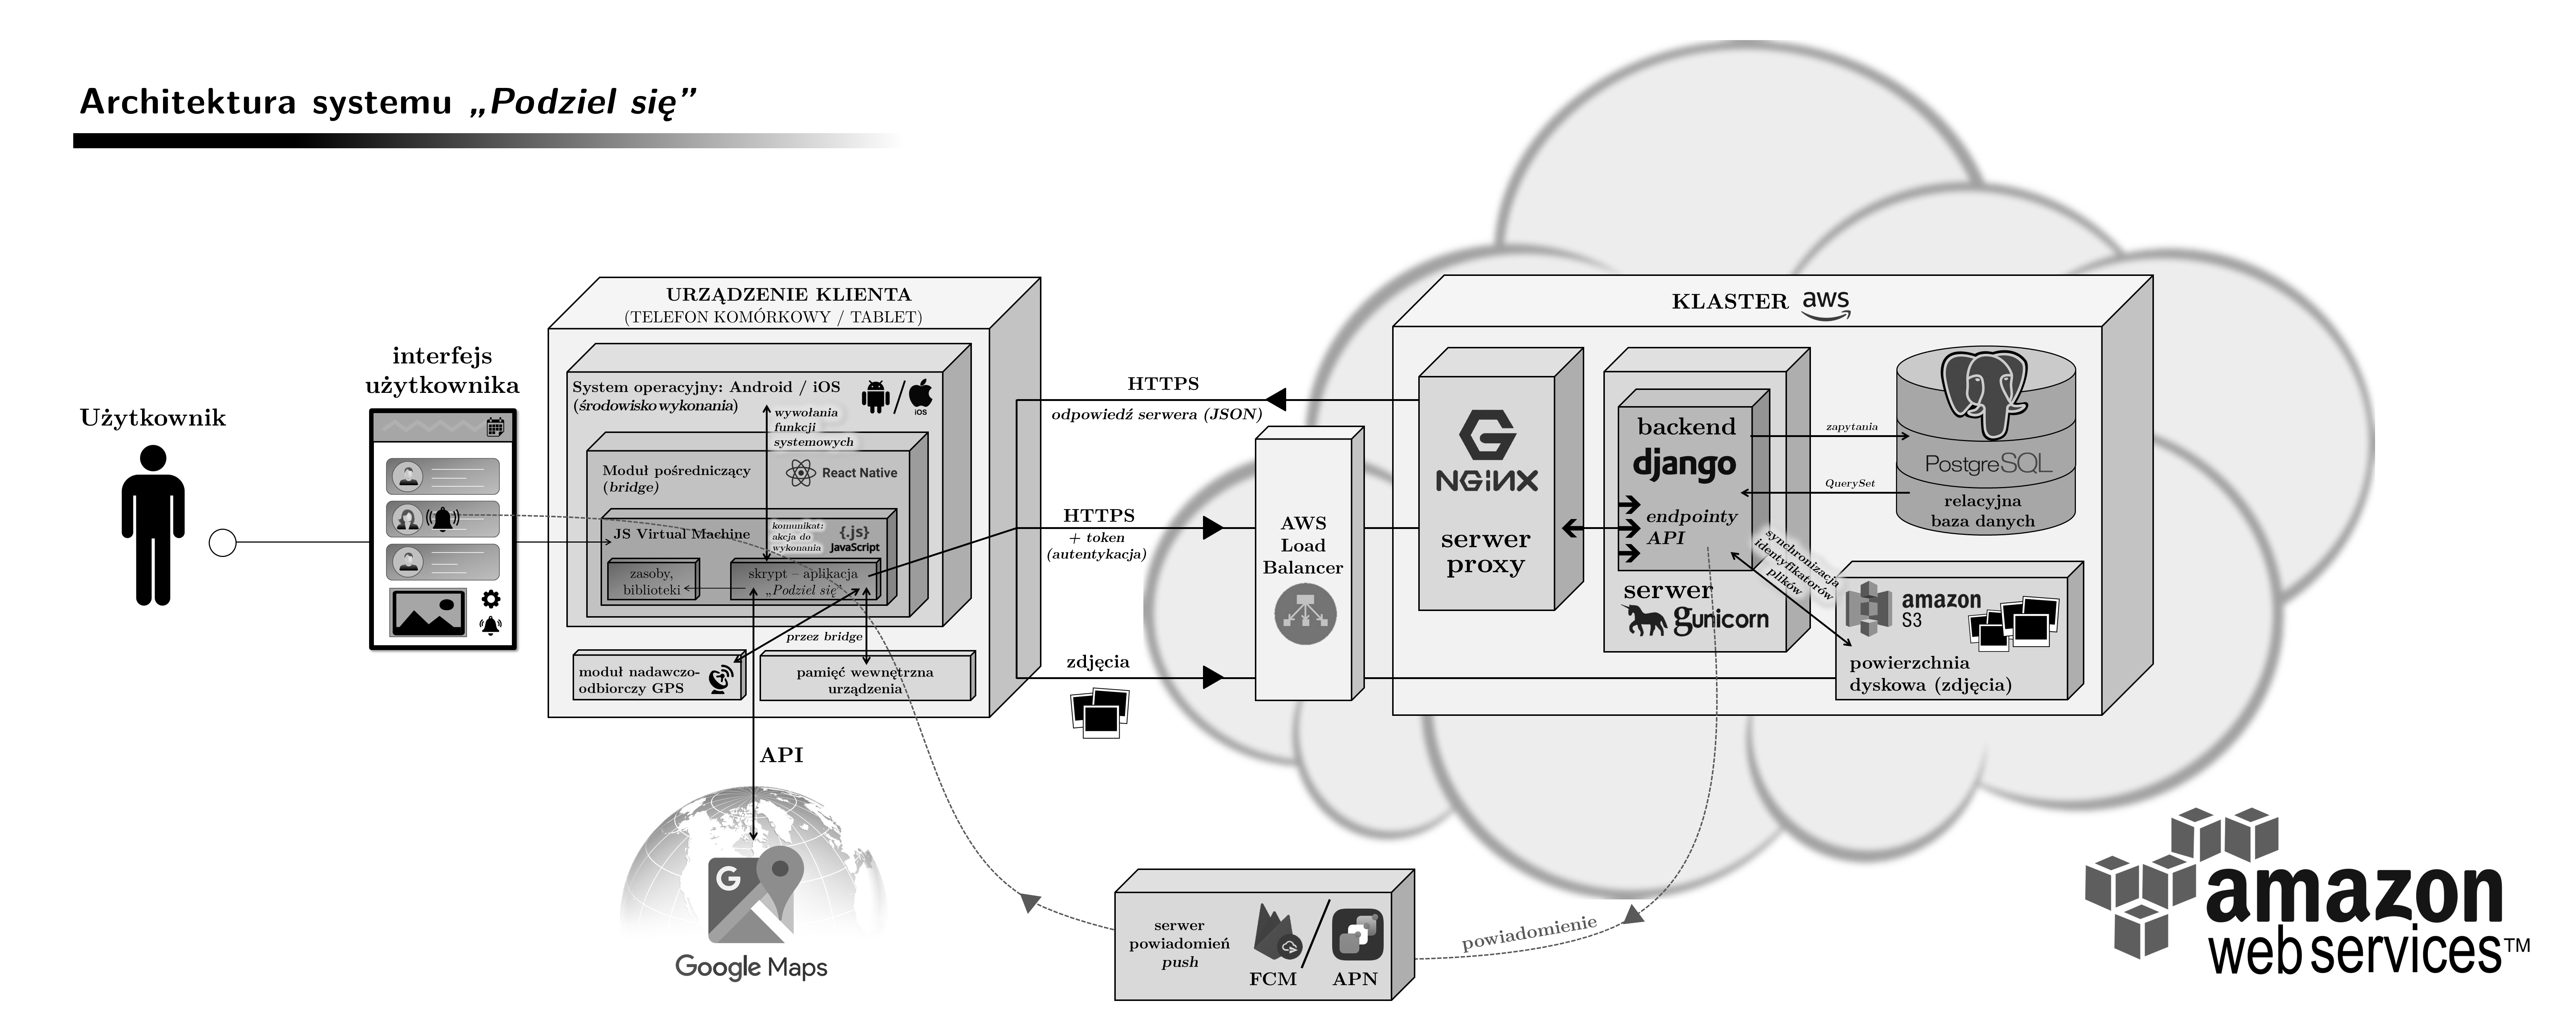
\includegraphics[width=\linewidth]{architektura.png}

\subsection{Aplikacja mobilna}
Aplikacja \textit{``Podziel się''} przeznaczona jest dla użytkowników dwóch najpopularniejszych mobilnych systemów operacyjnych: Androida oraz iOS\@. Interfejs aplikacji powstał z wykorzystaniem nowoczesnego frameworka React Native, pozwalającego opisać graficzne rozmieszczenie elementów na ekranie w składni zbliżonej do arkuszy stylów CSS, zaś logikę działania aplikacji w kodzie JavaScriptu. W React Native, przy użyciu specjalnego języka znaczników JSX, zostały zdefiniowane tzw.\ komponenty (lista ogłoszeń, przycisk wysyłania wiadomości, menu szufladkowe, okienko z komunikatem itp.), na bazie których React Native buduje komponenty natywne dla Androida oraz iOS\@. Pozwala to na ujednolicenie wyglądu interfejsu graficznego dla użytkowników różnych systemów i architektur --- aplikacja nie odbiega wyglądem od rozwiązań natywnych, projektowanych specjalnie z myślą~o~konkretnej platformie. Filozofia React Native polega na stosowaniu schematów tworzenia aplikacji webowych przy projektowaniu aplikacji działających w środowisku mobilnym, w szczególności możliwe jest korzystanie z rozmaitych pomocniczych bibliotek JavaScriptu.


Ważnym elementem React Native jest moduł pośredniczący (ang. \textit{bridge}), który tłumaczy wywołania pochodzące z wątków JavaScriptu na polecenia skierowane do systemu operacyjnego. Komunikaty opisujące akcje do wykonania są przesyłane w formacie JSON do modułu pośredniczącego, a po ich otrzymaniu \textit{bridge} wywołuje odpowiednie funkcje systemowe. Wymiana komunikatów jest asynchroniczna oraz nieblokująca, zatem React Native nie ingeruje nadmiernie w pracę systemu operacyjnego oraz umożliwia sprawne renderowanie widoków na ekranie. Co więcej, aplikacja ma możliwość swobodnej komunikacji ze środowiskiem wykonania; w razie potrzeby może uzyskać dostęp do modułu GPS, aparatu, pamięci wewnętrznej urządzenia itp.

\subsection{Część Serwerowa}

Cześć serwerowa została stworza w języku Python, w oparciu o framework Django. Pozwala on na szybkie tworzenie webowych interfejsów programistycznych aplikacji (po angielsku Web API) oraz łatwy dostęp do relacyjnych baz danych dzięki rozbudowanemu mechanizmowi mapowania obiektowo-relacyjnego (ORM). Polega ono na odwzorowaniu logicznych modeli encji, reprezentowanych jako klasy w języku Python, na rzeczywistą treść skryptów tworzących tabele i więzy spójności w bazie danych. Podobnie, wyniki zapytań są konwertowane do obiektu typu QuerySet, który może podlegać dalszemu przetwarzaniu przez serwer.

Jednym z głównych wymogów zamawiającej było stworzenie panelu administracyjnego. Wybrany framework umożliwa automatyczne generowanie panelu administratora. Wygenerowany panel umożliwia wykonywanie podstawowych operacji: pobierz, dodaj, usuń, modyfikuj na danych znajdujących się w bazie.

%Nie wiedziałem jak napisać to zdanie:
Do przychowywania danych wykorzystana została relacyjna baza danych PostegreSql z wtyczką PostGIS, która pozwala na wydajne wykonywanie zapytań zapytań przestrzennych. Zdjęcia zapisywane są w usłudze AmazonS3.

\subsection{Komunikacja Klient - Serwer}
Wymiana danych pomiędzy aplikacją mobilną a serwerem odbywa się za pomocą bezstanowego protokołu HTTP. Dane przesyłana są w formacie JSON, jest on formatem tekstowym i bazuje na podzbiorze języka JavaScript. Każde zapytanie do serwera uwierzytelniane jest unikalnym tokenem przyznwanym w momencie logowania bądź rejestracji, w związku z tym hasło użytkownika nie jest przechowywane w pamięci telefonu. Przy każdym ponownym logowaniu generowany jest nowy token.

Dane z serwera do urządzenia mobilnego (powiadomienia) wysyłane są natomiast za pośrednictwem usługi Firebase.

\section{PostGIS}
%liczenie odległosci itd.
Jedną z funkcjonalności naszej aplikacji jest prezentowanie użytkownikowi ofert z adresem odbioru w pobliżu jego aktualnej lokalizacji. Żeby to osiągnąć musieliśmy po stronie serwera być w stanie wyznaczyć wszystkie ogłoszenia z bazy danych, które są oddalone od zadanej lokalizacji nie więcej niż pewna wartość otrzymana w zapytaniu użytkownika. Pierwszym podejściem do rozwiązania tego problemu było wyznaczanie dla każdego zapytania wszystkich odległości pomiędzy adresem odbioru ogłoszeń a otrzymaną lokalizacją i wybranie tych, które są bliżej niż maksymalna odległość, którą wybrał użytkownik. Byłoby to jednak rozwiązanie bardzo nieefektywne, ponieważ dla każdego zapytania wymaga przejrzenia wszystkich ofert z bazy co przy większej ilości użytkowników i ofert może powodować problemy z wydajnością całego systemu.

Rozwiązaniem, na które ostatecznie się zdecydowaliśmy jest skorzystanie z rozszerzenia bazy danych PostgreSQL o nazwie PostGIS\@. Pozwala ono na wprowadzanie danych geograficznych do bazy i ich odpowiednią obsługę. Dla każdego ogłoszenia w bazie danych zapisujemy współrzędne geograficzne miejsca odbioru, dzięki czemu odpowiednia funkcja rozszerzenia PostGIS pozwala na znalezienie wszystkich ofert w ustalonej odległości od lokalizacji użytkownika. Operacja ta jest efektywna dlatego, że wyżej wspomniane rozszerzenie zmienia sposób przechowywania danych geograficznych w porównaniu do standardowej bazy danych. Zamiast B-drzewa używa R-drzewa, które jest strukturą danych wspomagającą wyszukiwanie obiektów w przestrzeni wielowymiarowej. Dla rzeczywistych danych to rozwiązanie jest dużo szybsze od podejścia naiwnego przedstawionego powyżej.

\section{Przechowywanie zdjęć}
%tutaj pasowało by napisać dlaczego nie składowanie danych na dysku

W trakcie tworzenia systemu, musieliśmy wybrać sposób przechowywania zdjęć. Pierwszym pomysłem było zapisywanie zdjęć na lokalnym dysku serwera. Szybko zdaliśmy sobie sprawę, że takie rozwiązanie posiada szereg wad. Pierwszą z nich jest brak elastyczności, w przypadku wyczerpania miejsca bylibyśmy zmuszeni zapłacić za droższy serwer, nawet jeżeli nie potrzebowalibyśmy szybszego procesora czy większej pamięci ram. Kolejną wadą jest duże obciążenia serwera, który musiałby obsłużyć zapytania HTTP związane z transferem tych zdjęć na urządzenia mobilne.

Zdecydowliśmy skorzystać z serwisu Amazon Simple Storage Service (Amazon S3). Usługa pozwala przechowywać dane w sposób trwały i bezpieczny. Zaletą Amazon S3 jest nieograniczona pojemność dyskowa oraz brak narzuconych limitów na transfer wychodzący. Co więcej, koszt usługi jest proporcjonalny do sumarycznego rozmiaru przechowywanych danych, mamy więc pełną elastyczność jeśli chodzi o koszty. Transfer plików jest szyfrowany protokołem SSL, ponadto same dane podlegają 256-bitowemu szyfrowaniu po stronie serwera.

Obsługa zdjęć zrealizowana jest w następujący sposób: Część mobilna kompresuje fotografie przed wysłaniem, następnie wysyła je w jednym zapytaniu wraz z informacjami o ogłoszeniu do serwera aplikacji \textit{``Podziel się''}. Serwer zapisuje dane ogłoszenia i metadane zdjęć w bazie PostegreSQL, a następnie wysyła obrazy do usługi Amazon S3. Przy pobieraniu informacji o dostępnych ogłoszeniach lub szczegółach danego ogłoszenia serwer zwraca odnośniki do zdjęć, następnie urządzenie mobilne pozyskuje dane bezpośrednio z serwisu Amazon S3. W ten sposób w znacznym stopniu redukowane jest obciążenia serwera aplikacji \textit{``Podziel się''}.

W dalszej perspektywie, w miarę rozwoju projektu, Amazon S3 oferuje rozszerzone plany wykorzystania oraz opcję archiwizacji danych z możliwością łatwego odtworzenia w przypadku nadpisania, usunięcia lub utracenia plików.

\section{Powiadomienia}
%tutaj dlaczego nie odpytywanie serwera non stop co jakiś czas

Aplikacja \textit{``Podziel się''} wspiera użytkowników w zarządzaniu licznymi ogłoszeniami wykorzystując mechaniz powiadomień. Wspomniana funkcjonalność pozwala na wyświetlanie użytkownikom krótkich komunikatów o zajściu zdarzeń wymagających uwagi.

Powiadomienia wyświetlane są w przypadku zajaścia jednego z następujących zdarzeń:
\begin{itemize}
\setlength\itemsep{-0.2em}
    \item otrzymanie wiadomości od innego użytkownika,
    \item dodanie nowego ogłoszenia w okolicy,
    \item dodanie nowego ogłoszenia przez obserwowaną osobę
    \item polubienie naszego ogłoszenia,
\end{itemize}{}

Najprostszym sposobem implementacji tej funkcjonalności jest regularne odpytywanie serwera czy są dostępne nowe powiadomienia. Jednakże ze względu na ograniczenia systemu Android jak i IOS, obsługa procesów w tle (to znaczy wtedy kiedy użytkownik nie korzysta z aplikacji) jest bardzo mocno ograniczona. Procesy w tle nie mogą być uruchamiane częściej niż co kilkadziesięt minut. Związane jest to z oszcządzaniem energi.

Z tego względu zdecydowaliśmy się na użycie zewnętrznych usług takich jak: Firabase Cloud Messaging (FCM), dla systemu Androida oraz Apple Push Notification (APN) w przypadku IOS\@. Umożliwiają one niemalże natychmiastowe dostarczanie wiadomości z serwera do telefonu użytkownika.

Schemat działania systemu powiadomień wygląda następująco: urządzenie mobilne przy pierwszym uruchomieniu pobiera unikalny identyfkiator (token) z serwisu FCM bądź APN, jest on wysyłany na serwer aplikacji \textit{``Podziel się''} w trakcie logowanie lub rejestracji, a następnie zapisywany w bazie danych. W przypadku potrzeby dostarczenia powiadomienia na dane urządzenie, serwer aplikacji \textit{``Podziel się''} wyśle do serwera FCM wiadomość zawierającą token danego telefonu oraz zawartość powiadomienia. Usługa FCM przekieruje notyfikację do konkretnego użytkownika na podstawie denego identyfikatora urządzenia. Zachowanie telefonu lub tabletu po odebraniu nowego powiadomienia zależy od preferencji użytkownika, może to być okienko z wiadomością, sygnał dźwiękowy lub ikonka na ekranie.

Udało nam się zaimplementować w pełni funkcjonalne rozwiązanie na platformie Android. Jeśli chodzi o system IOS to wymogiem usługi APN było posiadanie konta w programie \textit{Apple Developer Program}. Niestety ze wzlędów czasowych i formalnych nie byliśmy w stanie przystąpić do tego programu. Jednakże zarówno aplikacja mobilna jak i część serwerowa są już przystosowane do obsługi APN, wystarczy jedynie odpowiednio skonfigurwać platformę Firebase (wgrać odpowiednie certyfikaty wygenerowane na koncie dewelopera Apple), wtedy powiadomienia do użytkowników Apple będę przekierowywane do APN\@.

\section{Logowanie za pomocą Facebooka}
%dlaczego to jest wygodne, jak działa itd...
Oprócz klasycznej możliwości logowania poprzez podanie adresu e-mail i hasła zgodnych z tymi zapisanymi podczas rejestracji, istnieje także opcja zalogowania przez połączenie swojego konta w serwisie Facebook z kontem w aplikacji \textit{Podziel się}. Cały proces z punktu widzenia użytkownika polega na naciśnięciu przycisku logowania z Facebookiem na ekranie logowania, udzieleniu odpowiednich pozwoleń i zalogowaniu się do swojego konta w serwisie Facebook. Po wykonaniu tych czynności użytkownik może już korzystać z aplikacji, co więcej jego dane i zdjęcie profilowe zostaną automatycznie pobrane. Taka możliwość pozwala na jeszcze szybsze skorzystanie z aplikacji \textit{Podziel się} niż klasyczne logowanie.

Funkcjonalność ta jest możliwa dzięki modułowi integrującemu aplikację napisaną z użyciem React Native z kontem w serwisie Facebook. Po udzieleniu potrzebnych pozwoleń i zalogowaniu użytkownika do konta Facebook, aplikacja \textit{Podziel się} pobiera klucz pozwalający na zidentyfikowanie użytkownika. Następnie uzyskany klucz jest przesyłany do serwera, gdzie jest weryfikowany i na jego podstawie, a także osobnego klucza specyficznego dla całej aplikacji, pobierane są dane użytkownika takie jak: imię, nazwisko, zdjęcie profilowe, identyfikator użytkownika. Potem sprawdzane jest czy ten użytkownik posiada już konto, jeżeli nie to jego dane dodawane są do bazy danych, a następnie do urządzenia mobilnego wysyłany jest token uwierzytelniający --- analogicznie jak przy klasycznym logowaniu.

\section{Działanie aplikacji mobilnej na dwóch systemach operacyjnych}
%opis że było wszystko działa na ios i że ogóle spoko
%nie wiem jak to ładnie nazwać
System operacyjny Android jest niezwykle popularny w naszym kraju. Według IDC 91,5\% sprzedanych smarfonów w 2017 roku stanowiły urządzenia działające pod kontrolą systemu firmy Google (patrz~\cite{popluarnoscAndroid}).

Z tego względu postanowiliśmy, że w pierwszej kolejności tworzymy aplikację na platformę Android, a dopiero później zajmiemy się systemem IOS\@. W trakcie pracy nad wersją androidową używaliśmy tylko i wyłącznie bibliotek, których twórcy wyraźnie informowali o komaptybilności z obydwoma systemami. Pozwoliło nam to dosyć bezboleśnie uruchomić aplikację na symulatorze iPhone.

Nie udało nam się jedynie zaimplementować dwóch funkcjonalności:

Pierwszą z nich jest logowanie z Facebookiem. Pomimo tego, że twórcy biblioteki z której skorzystaliśmy, zapewniali o działaniu na platformie IOS, to nie udało nam się odpowiednio jej skonfigurwać do działałania z naszą aplikacją.

Drugą są powiadomienia. Tak jak pisaliśmy we wcześniejszym podrozdziale, wymogiem było posiadanie konta w programie \textit{Apple Developer Program}.

Cała pozostała funkcjonalność działa dokładnie tak jak na systemie firmy Google. W szczególności, obie wersją mają taki sam interfejs użytkownika. Różni on się jedynie szczegółami, typowymi dla danej platformy. Na przykład komponentami wyboru daty lub zdjęć z galerii. Poniżej zrzuty tych samych ekranów aplikacji, wykonane odpowiednio na emulatorze Android i symulatorze iPhone:

\newpage
\begin{figure}[h!]
  \centering
  \begin{subfigure}[b]{0.4\linewidth}
    \begin{framed}
      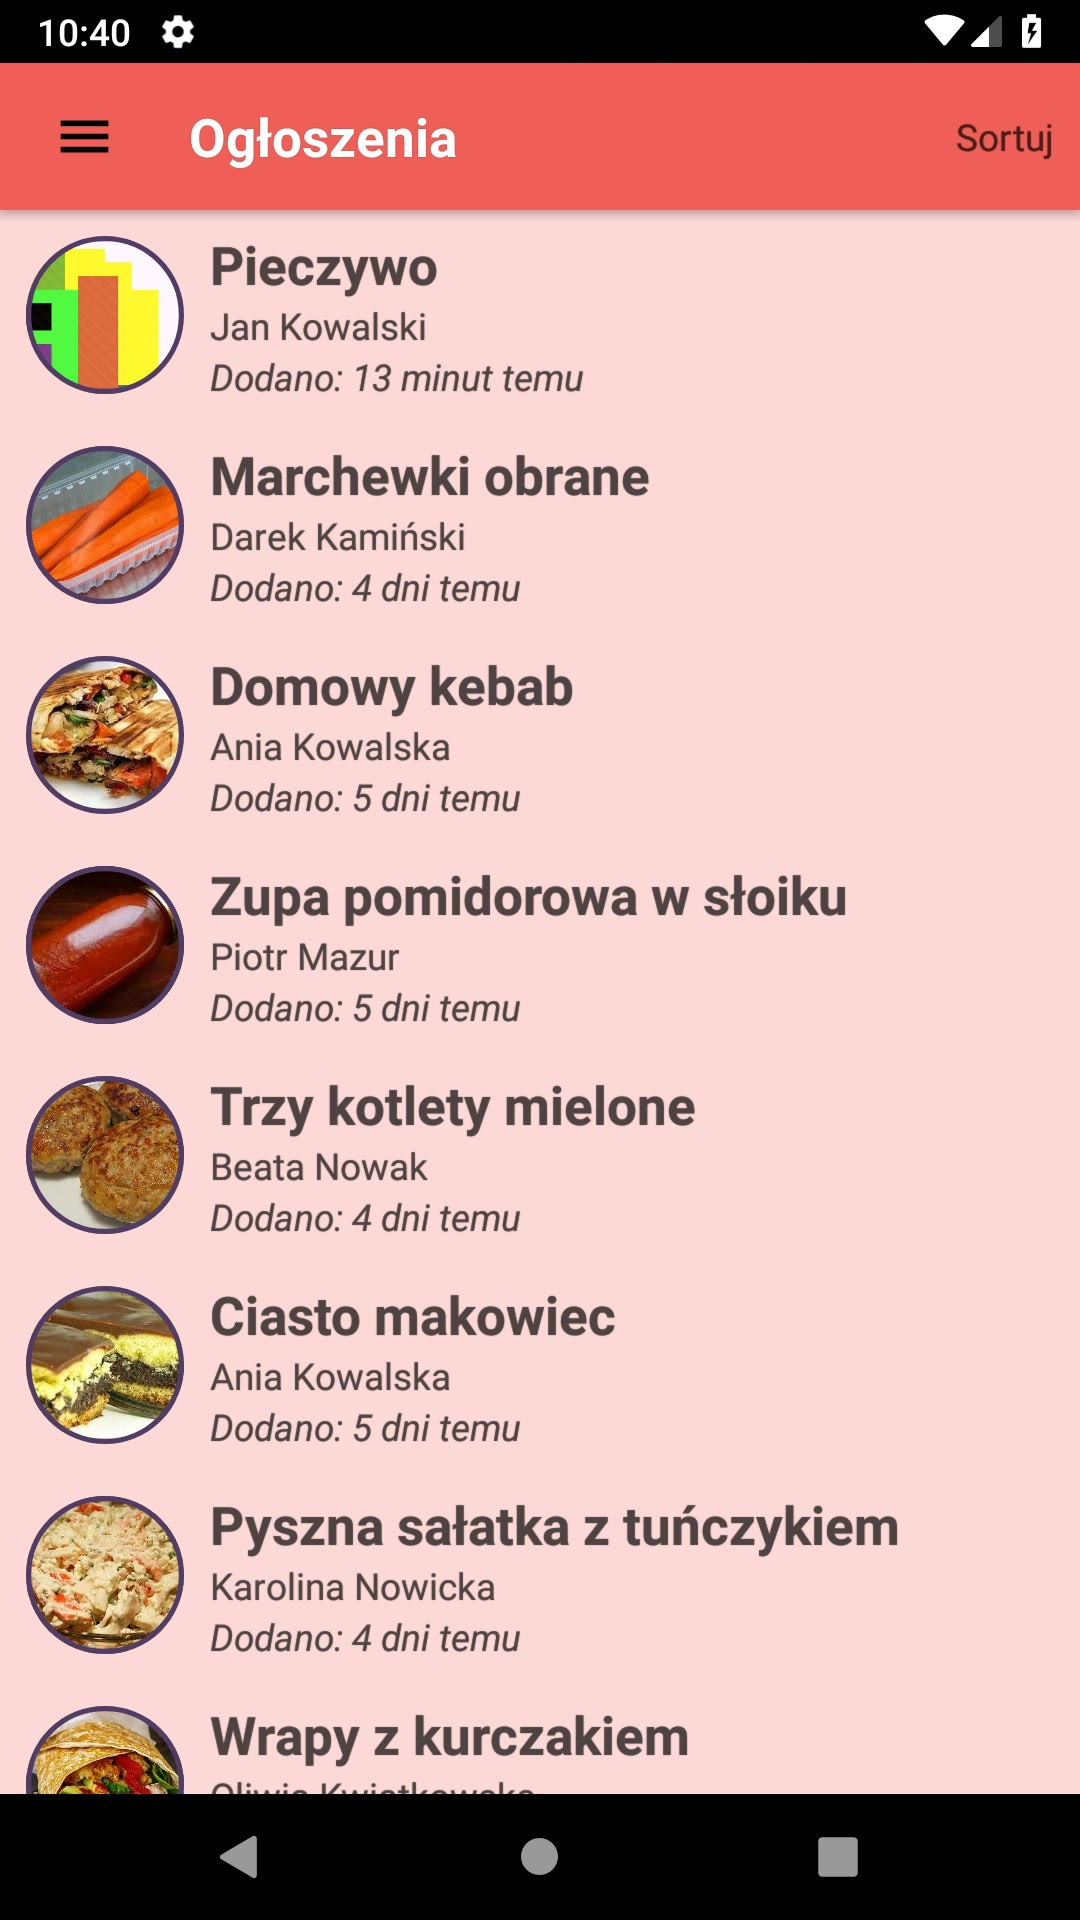
\includegraphics[width=\linewidth]{android1.jpg}
    \end{framed}
    \caption{Android.}
  \end{subfigure}
  \begin{subfigure}[b]{0.4\linewidth}
    \begin{framed}
      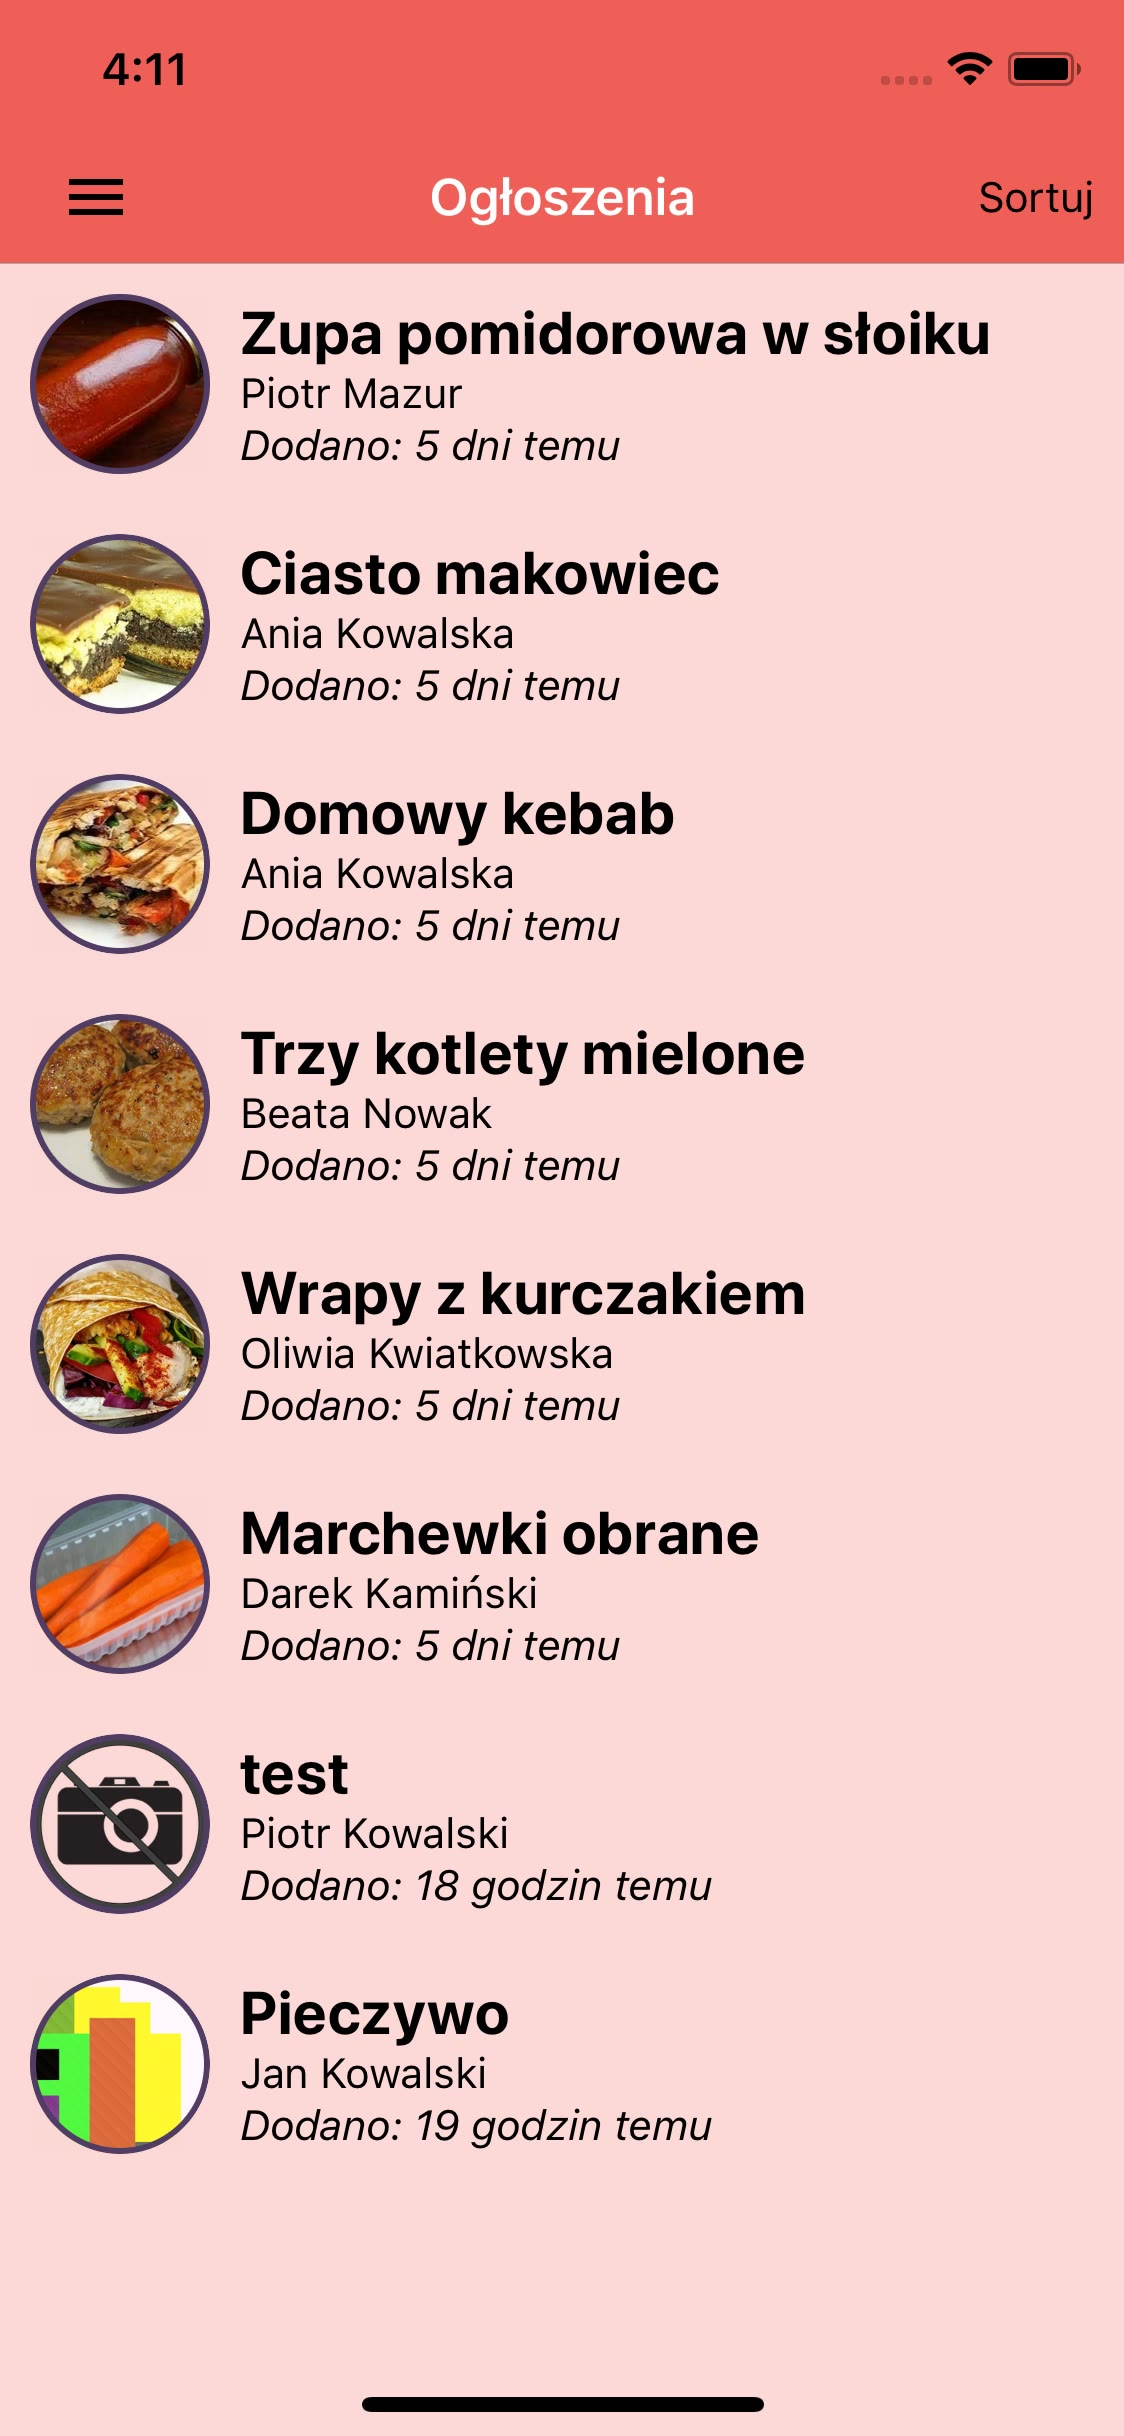
\includegraphics[width=\linewidth]{ios1.jpg}
    \end{framed}
    \caption{iPhone.}
  \end{subfigure}
  \caption{Lista ogłoszeń.}
  \label{fig:offers}
\end{figure}

\newpage
\begin{figure}[h!]
  \centering
  \begin{subfigure}[b]{0.4\linewidth}
    \begin{framed}
      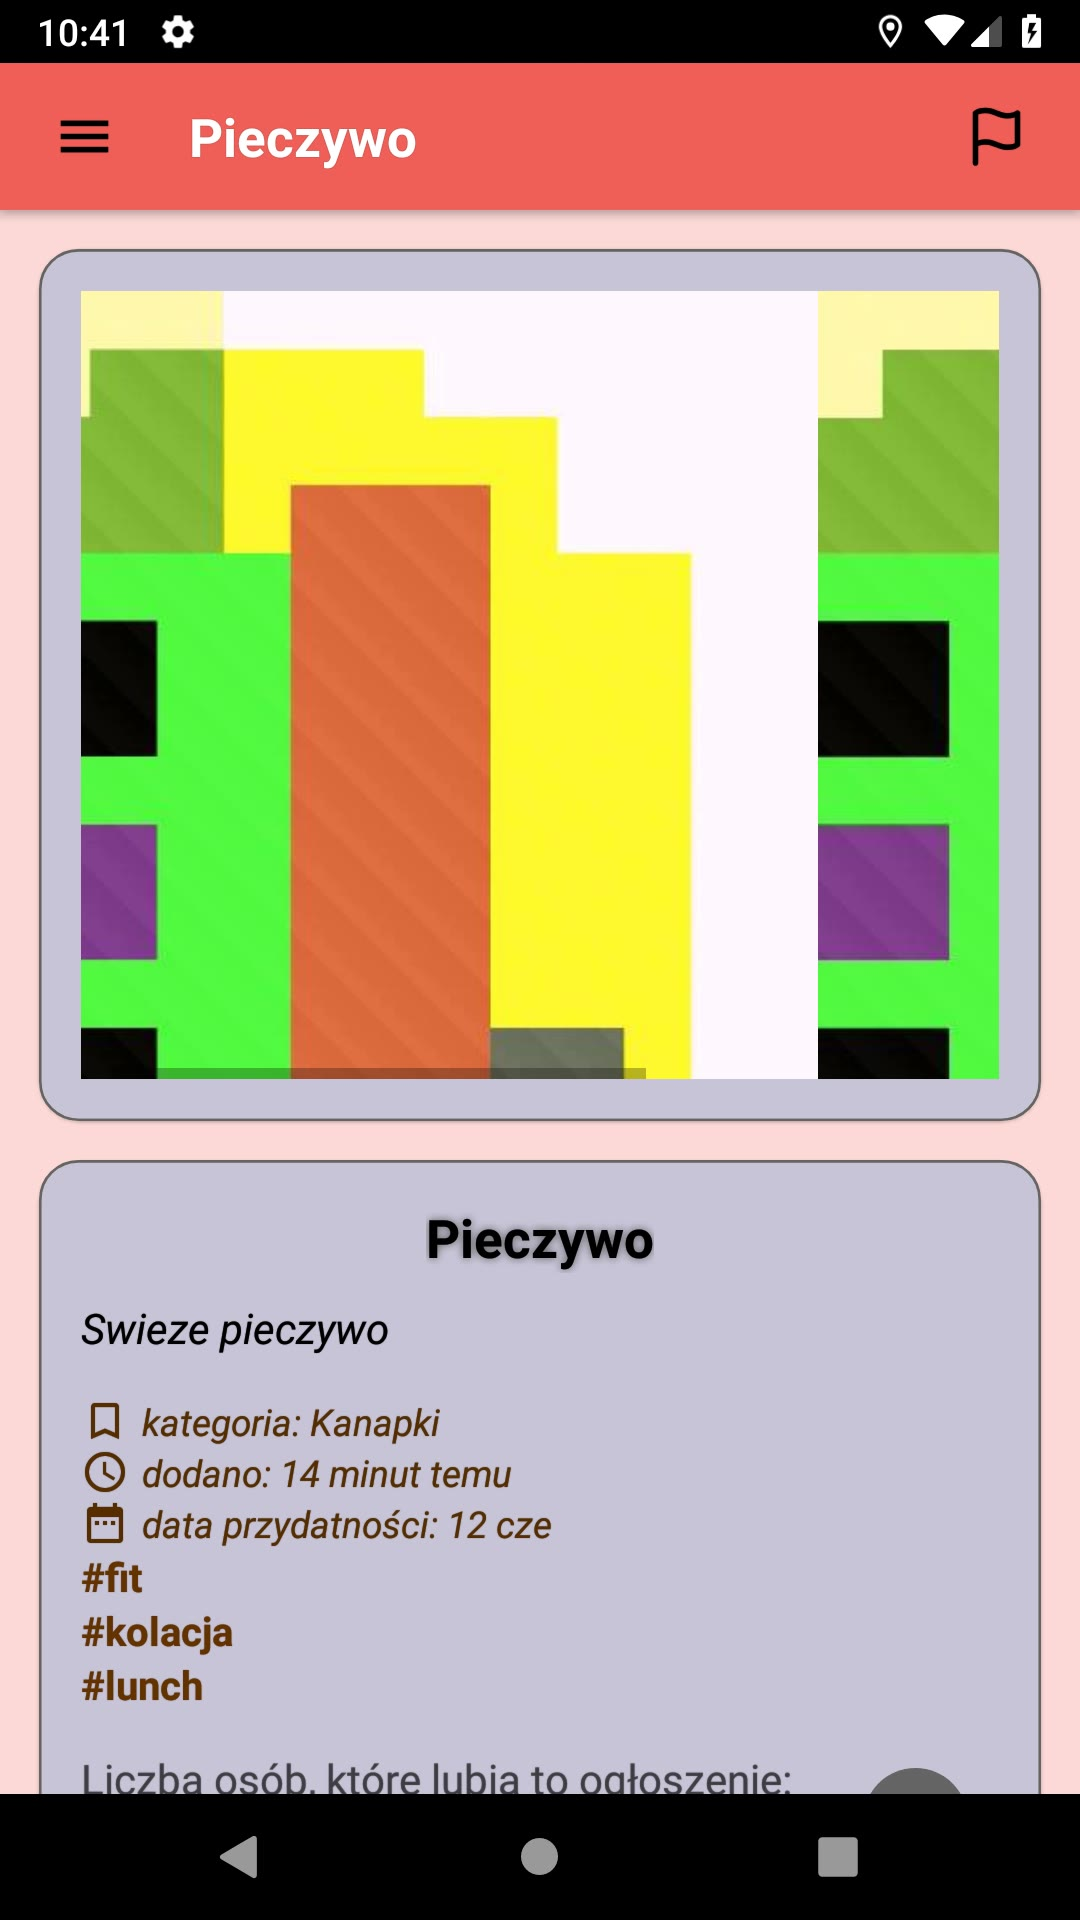
\includegraphics[width=\linewidth]{android2.jpg}
    \end{framed}
    \caption{Android.}
  \end{subfigure}
  \begin{subfigure}[b]{0.4\linewidth}
    \begin{framed}
      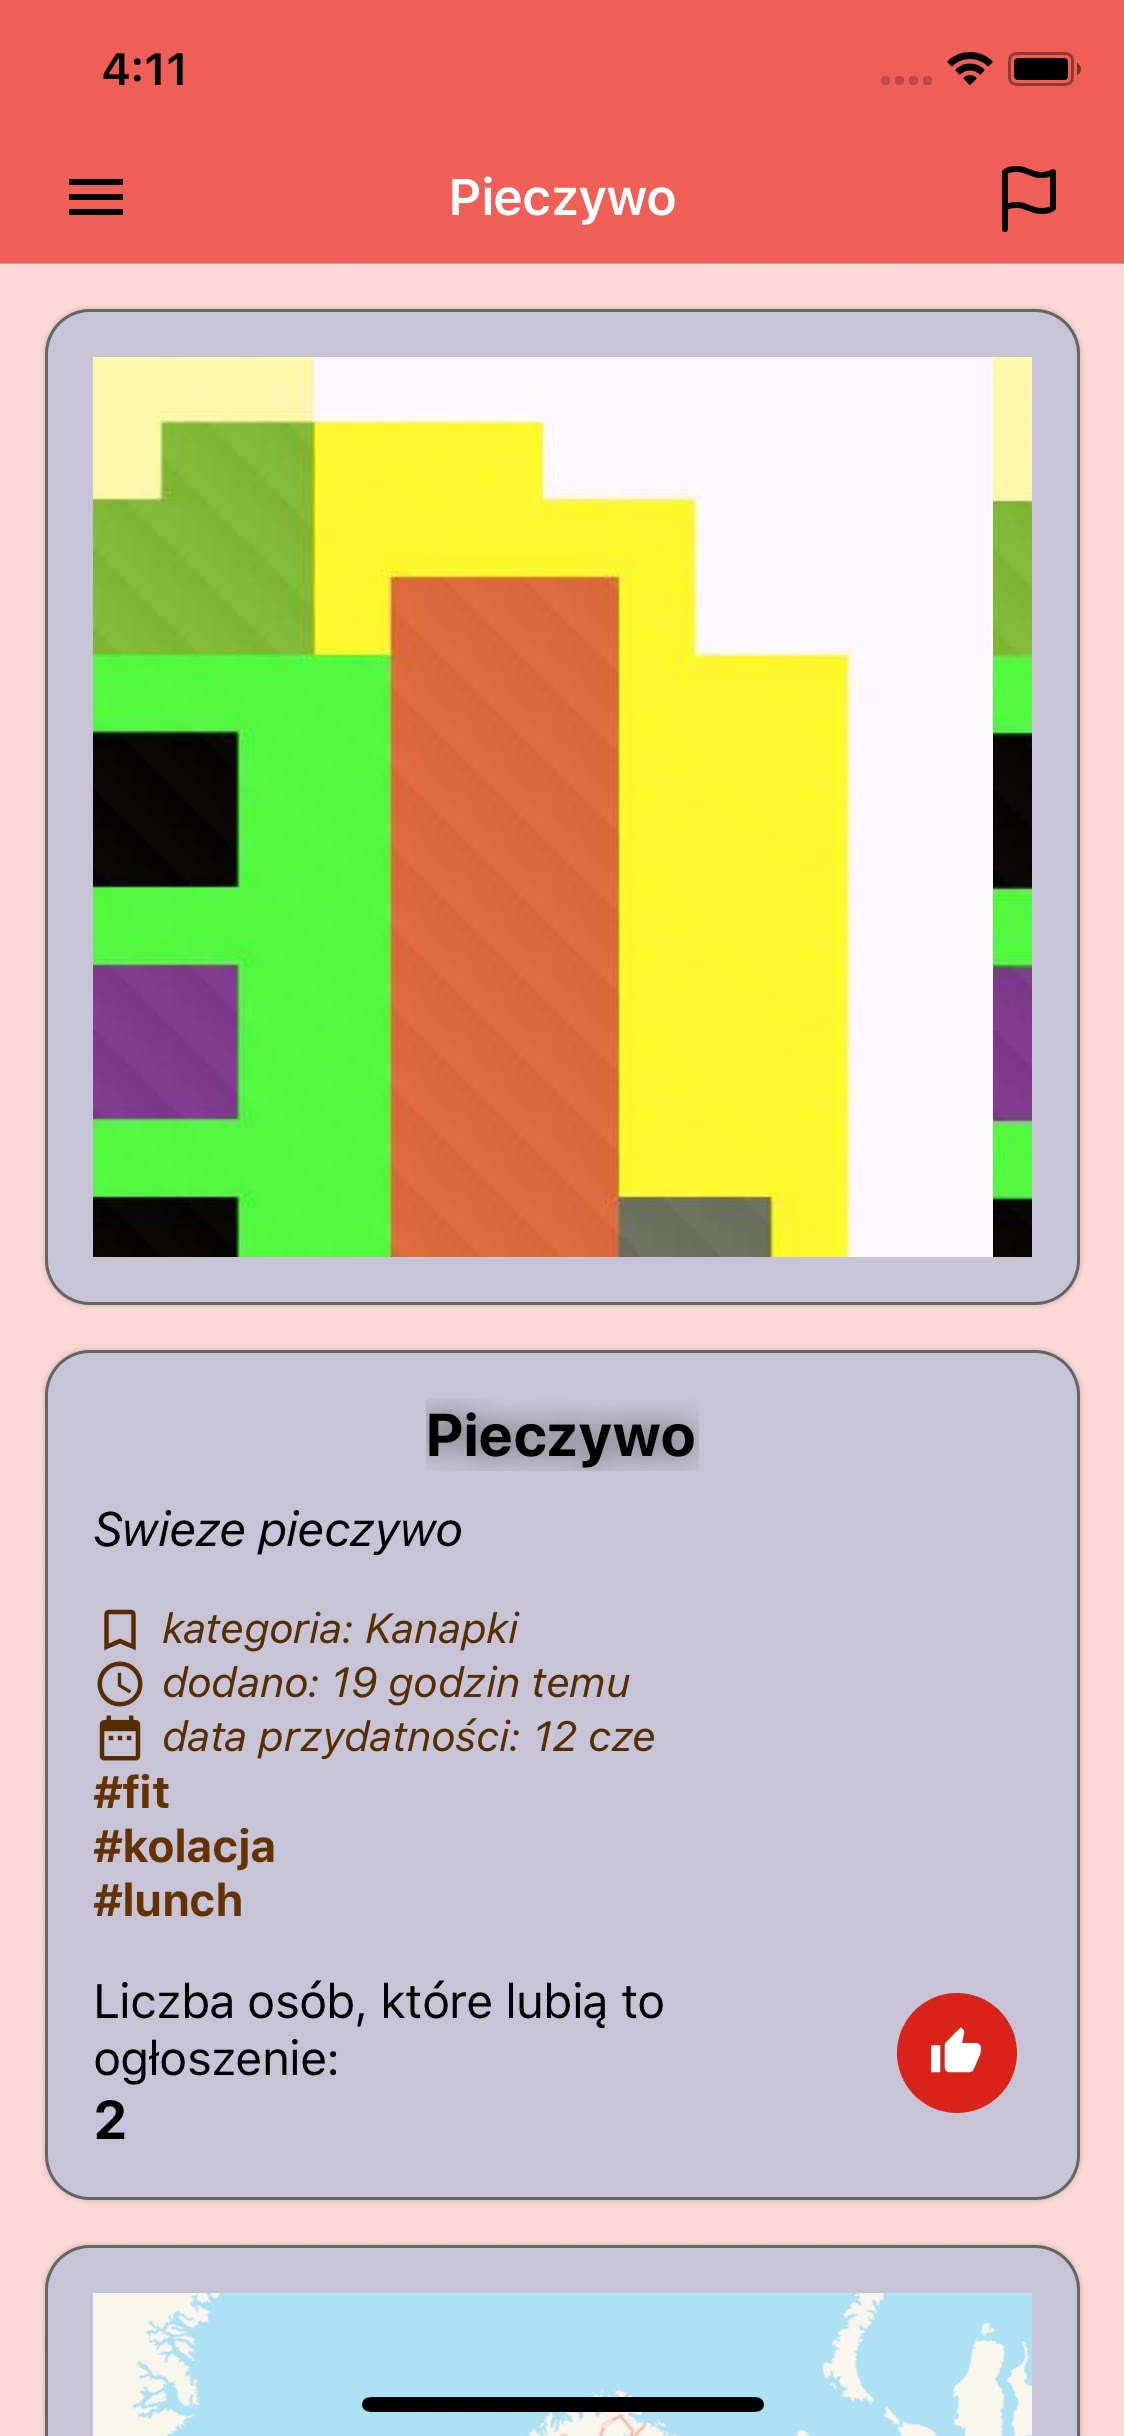
\includegraphics[width=\linewidth]{ios2.jpg}
    \end{framed}
    \caption{iPhone.}
  \end{subfigure}
  \caption{Szczegóły ogłoszenia.}
  \label{fig:offer}
\end{figure}

\newpage
\begin{figure}[h!]
  \centering
  \begin{subfigure}[b]{0.4\linewidth}
    \begin{framed}
      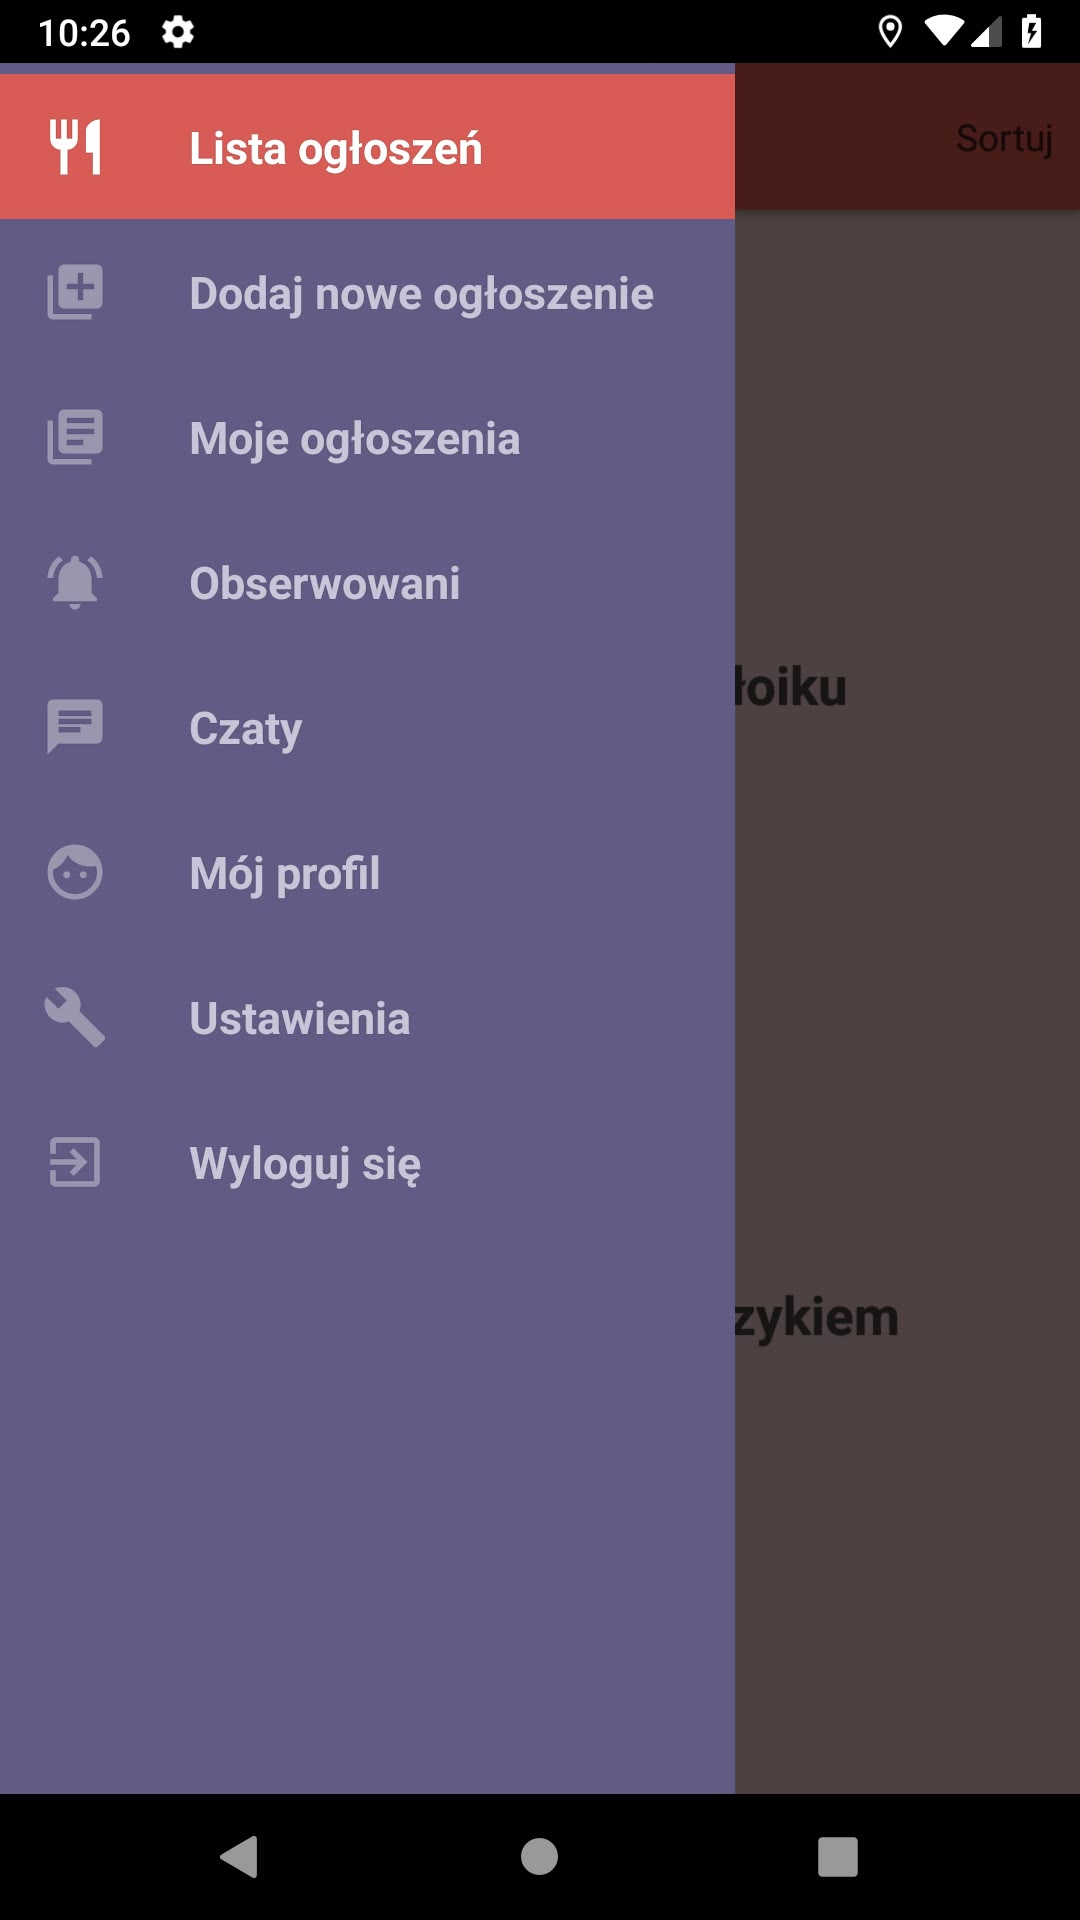
\includegraphics[width=\linewidth]{android3.jpg}
    \end{framed}
    \caption{Android.}
  \end{subfigure}
  \begin{subfigure}[b]{0.4\linewidth}
    \begin{framed}
     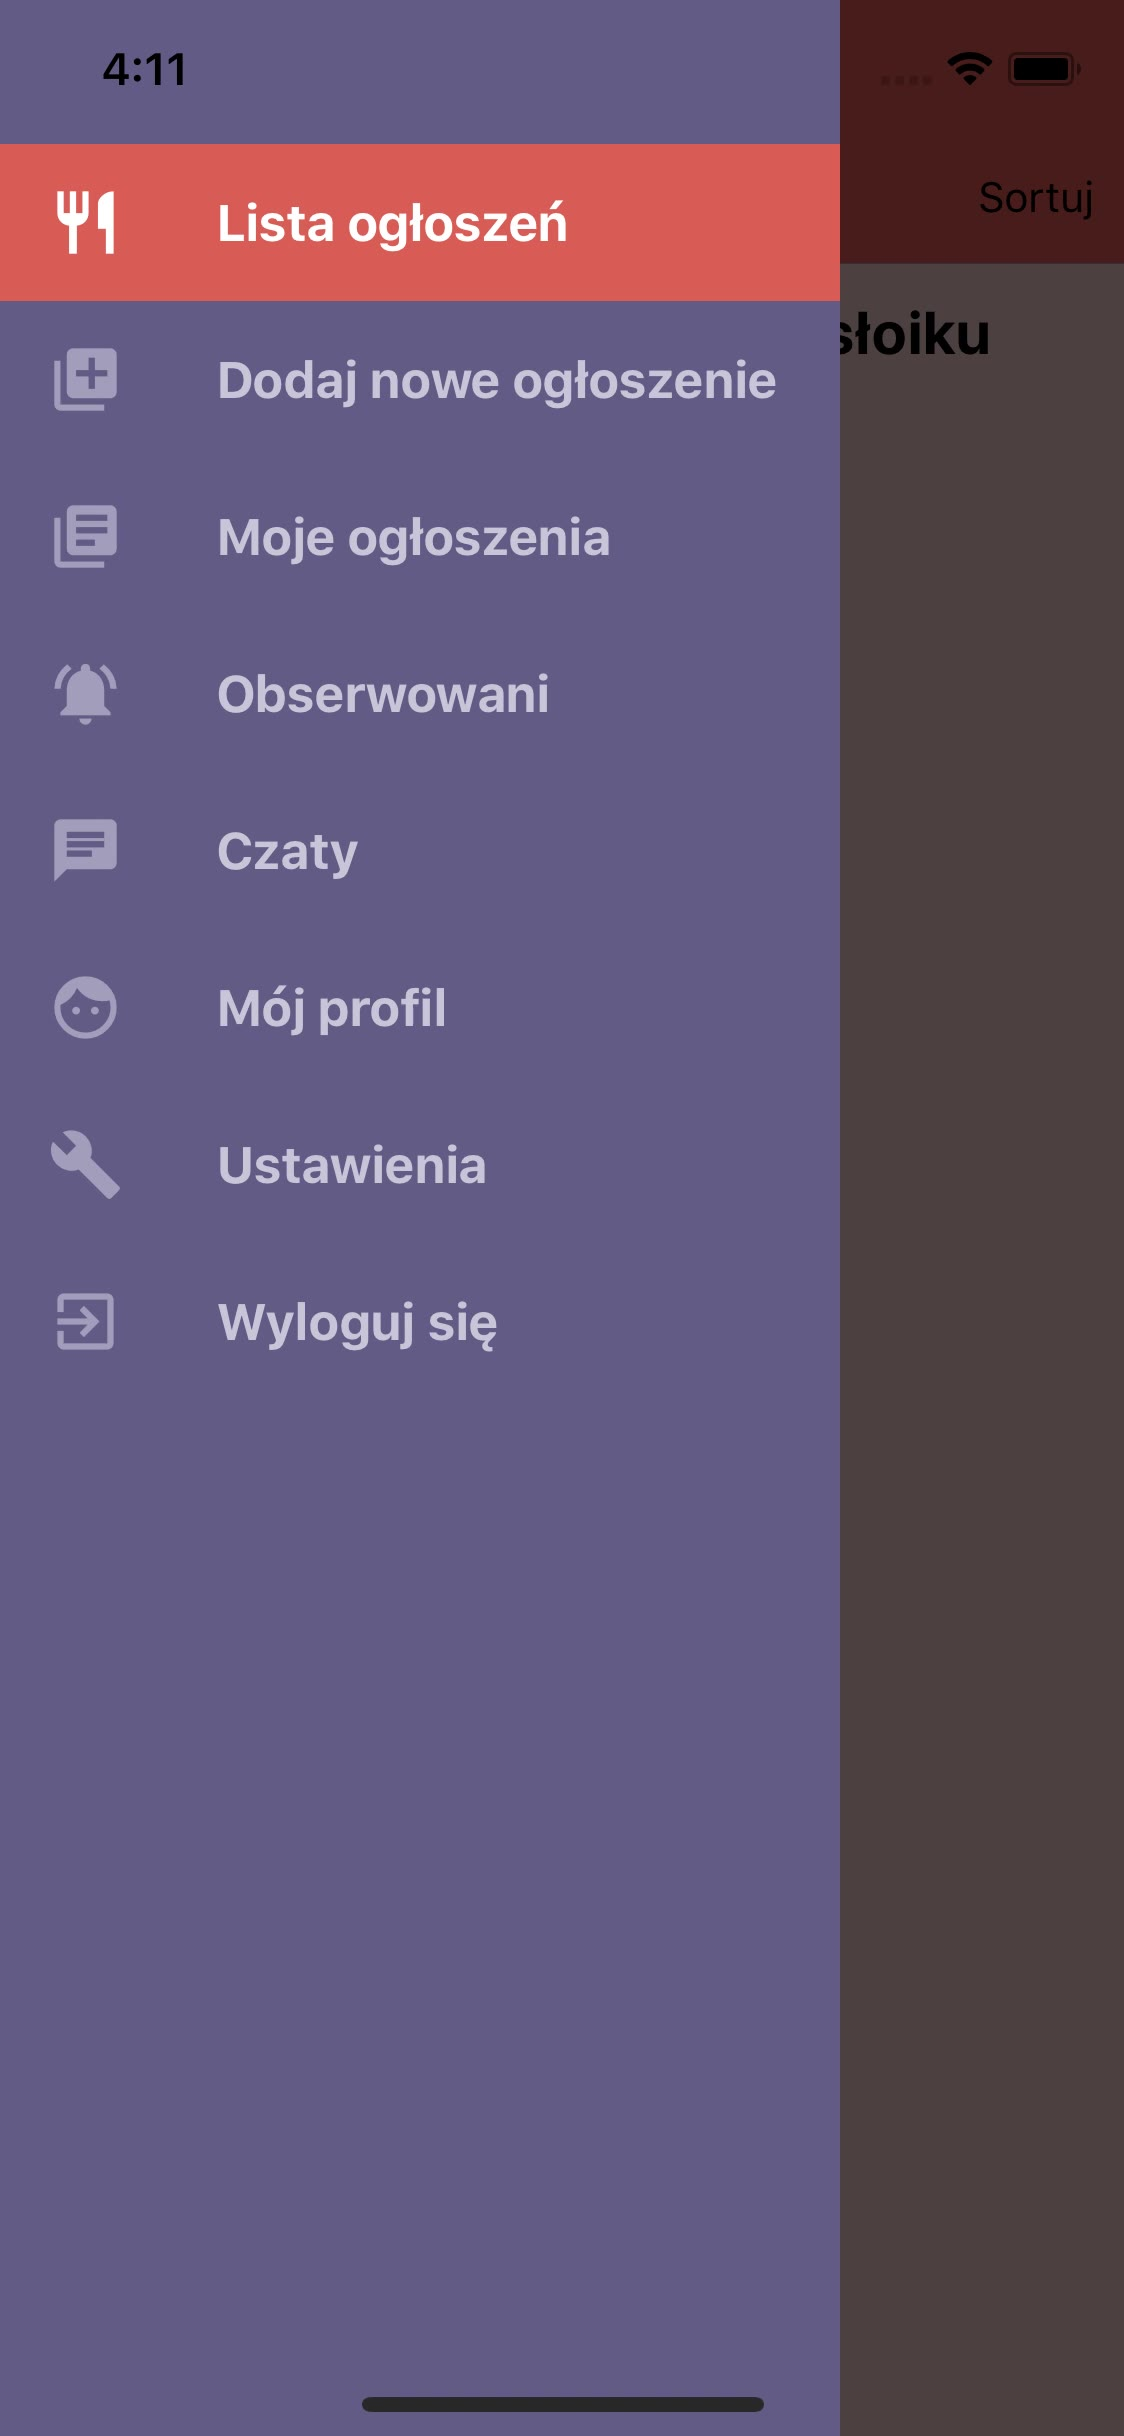
\includegraphics[width=\linewidth]{ios3.jpg}
    \end{framed}
    \caption{iPhone.}
  \end{subfigure}
  \caption{Menu główne.}
  \label{fig:menu}
\end{figure}

\newpage

\chapter{Infrastruktura serwera}\label{r:infrastruktura}

Potrzeba udostępnienia pierwszej wersji aplikacji zamawiającemu, postawiła nas przed koniecznością uruchomienia stałego serwera aplikacyjnego. Musieliśmy podjęć decyzję dotycząca wyboru platformy na której będzie uruchomiony nasz serwer. Ze względu na bardzo dużo liczbę firm oferujących usługi typu wirtualny prywatny serwer, nie był to łatwy wybór.

\section{Kryteria}
Przy wyborze usługodawcy kierowaliśmy się następującymi kryteriami:
\begin{itemize}
    \item \textbf{Cena} --- w trakcie tworzenia systemu z aplikacji korzystało tylko kilka osób: nasz zespół i
    zamawiający, niepotrzebowaliśmy więc drogiego i bardzo wydajnego serwera,
    \item \textbf{Skalowalność} --- chcieliśmy mieć możliwość łatwego zwiększenia dostępnych zasobów jeśli
    zwiększy się liczba osób korzystających z systemu,
    \item \textbf{System operacyjny Linux} --- wybrany serwer powinien działać w oparciu o jedną z dystrybucji
    systemu Linux,
    \item \textbf{Prosta administracja} --- nikt z nas nie miał wcześniej doświadczenia związanego z administrowaniem serwerem, wybrany serwis musiał być więc dostatecznie prosty w obsłudze,
\end{itemize}{}

\section{Amazon Lightsail}

Nasz wybór padł na usługę \textit{``Lightsail''} firmy Amazon. Decyzja o wybraniu produktu firmy Amazon została podjęta z uwagi na jej wydajność, skalowalność, stosunkowo niską awaryjność, akceptowalną cenę (3,5\$ kosztuje najtańszy pakiet miesięcznie) oraz obecność rozbudowanych mechanizmów zapewniających bezpieczeństwo danych. Lightsail udostępnia maszynę wirtualną działającą pod kontrolą systemu Linux Ubuntu, ze statycznym adresem IP\@.

Administracja jest możliwa za pomocą witryny internetowej. Możliwe jest między innymi: zresetowanie maszyny, reinstalacja systemu czy wykonanie i przywrócenie kopi zapasowej.

\section{Oprogramowanie serwera}

Część serwerowa aplikacji działa pod kontrolą serwera HTTP Gunicorn. Gunicorn odpowiada za wykonanie odpowiedniego kodu języka Python oraz współpracę z serwerem pośredniczącym nginx. Nginx odbiera połączenia od klientów oraz obsługuje statyczne zapytania HTTP, zaś dynamiczne przekierowuje do Gunicorna i Django z wykorzystaniem standardu WSGI (Web Server Gateway Interface). Po otrzymaniu odpowiedzi nginx odsyła klientowi wynik zapytania. Wprowadzenie serwera proxy pozwala na łatwiejszą regulację obciążenia oraz zapobieganie opóźnieniom wynikającym z konieczności obsługi klientów dysponującym powolnym połączeniem internetowym.

Baza danych PostegreSQL wraz z wtyczką PostGIS uruchomiona jest kontenerze Docker.

\section{Dostęp do Serwera}
Połączenie z serwerem odbywa się za pomocą protokołu SSH\@. Możliwy jest również dostęp za pomocą konsoli dostępnej na stronie internetowej serwisu Lightsail.

\section{Dalszy rozwój}
W miarę dalczego rozwoju projektu, narzędzie firmy Amazon oferuje elastyczne plany, zawierajęce większą liczbę rdzeni procesore, pamięci ram czy przestrzeni dyskowej. Istniej również możliwość łatwej integracji z innymi produktami z rodziny Amazon Web Services (AWS) takimi jak na przykład dedykowane serwery do równoważenia obciążenia, narzędzia do zarządzania domenami i certyfikatami SSL\@.


\chapter{Przypadki użycia}\label{r:usecase}
Niniejszy rozdział prezentuje kluczowe przypadki użycia aplikacji, ze szczególnym uwzględnieniem interakcji pomiędzy użytkownikiem a komponentami systemu. Przedstawione zostały również ścieżki alternatywne, a także dodatkowe funkcjonalności, o które można wzbogacić aplikację w dalszej perspektywie czasowej.

\section{Rejestracja}
    \subsection{Krótki opis}
    Utworzenie nowego konta użytkownika w aplikacji.
    \subsection{Cele}
    \begin{itemize}
    \item Umożliwienie aplikacji identyfikacji użytkowników w celu dostarczenia im określonych funkcjonalności.
    \item Uzyskanie informacji koniecznych do poprawnego działania aplikacji.
    \end{itemize}
    \subsection{Warunki wstępne}
    \begin{itemize}
        \item Aplikacja jest zainstalowana na urządzeniu użytkownika.
        \item Użytkownik dysponuje stałym połączeniem internetowym.
    \end{itemize}
    \subsection{Czynności}
    \subsubsection{Czynności podstawowe}
    \begin{enumerate}
        \item Użytkownik naciska przycisk ``Załóż nowe konto''.
        \item Aplikacja wyświetla użytkownikowi formularz rejestracyjny.
        \item Użytkownik wprowadza swoje imię, nazwisko, adres e-mail, hasło.
        \item W polu ``Powtórz hasło'' użytkownik wpisuje drugi raz to samo hasło.
        \item Użytkownik naciska przycisk ``Utwórz konto''.
        \item Aplikacja potwierdza poprawną rejestrację.
        \item Następuje przejście do ekranu dodawania zdjęcia profilowego. Początkowo widoczny jest domyślny awatar.
            \begin{itemize}
                \item Jeżeli użytkownik nie chce zamieścić własnego zdjęcia, naciska przycisk ``Dalej''.
                \item W przypadku wskazania opcji ``Zmień zdjęcie profilowe'' aplikacja wyświetla okienko z prośbą o wskazanie źródła zdjęcia, do wyboru: załączenie zdjęcia z pamięci urządzenia (galerii) lub utworzenie aparatem nowego zdjęcia.
                    \begin{itemize}
                        \item Jeżeli użytkownik wyrazi chęć dodania istniejącego zdjęcia, aplikacja uruchamia klasyczny interfejs przeglądania galerii systemu operacyjnego.
                        \item Wybór opcji zrobienia nowego zdjęcia przekazuje sterowanie wbudowanej w~system operacyjny aplikacji obsługującej aparat.
                    \end{itemize}
            \end{itemize}
     \item Aplikacja pyta użytkownika, czy chce korzystać z usługi geolokalizacji do sortowania listy ogłoszeń względem aktualnego położenia.
     \item Użytkownik wyraża zgodę na korzystanie z geolokalizacji.
     \item Proces rejestracji został zakończony --- użytkownik jest domyślnie zalogowany do aplikacji na danym urządzeniu.
    \end{enumerate}
    \subsubsection{Czynności alternatywne}
    \begin{enumerate}
        \item Jeśli użytkownik wypełnił formularz w sposób niepoprawny:
        \begin{itemize}
            \item za drugim razem wprowadził inne hasło,
            \item nie wypełnił któregoś z pól,
            \item wprowadził niepoprawny składniowo adres e-mail,
        \end{itemize}
        aplikacja powiadamia użytkownika o popełnionym błędzie i odsyła go z powrotem do edycji formularza.
        \item Jeżeli użytkownik nie wyraził zgody na korzystanie z geolokalizacji, aplikacja pyta użytkownika, względem jakiego miejsca ma sortować ogłoszenia i wyświetla interaktywną mapę. Aby kontynuować, użytkownik musi wskazać konkretne miejsce na mapie.
    \end{enumerate}

\newpage
\begin{figure}[H]
  \centering

  \begin{subfigure}[b]{0.4\linewidth}
    \begin{framed}
      
\includegraphics[width=\linewidth]{rejestracja1.png}
    \end{framed}
    \caption{Ekran powitalny.}
  \end{subfigure}
  \begin{subfigure}[b]{0.4\linewidth}
    \begin{framed}
      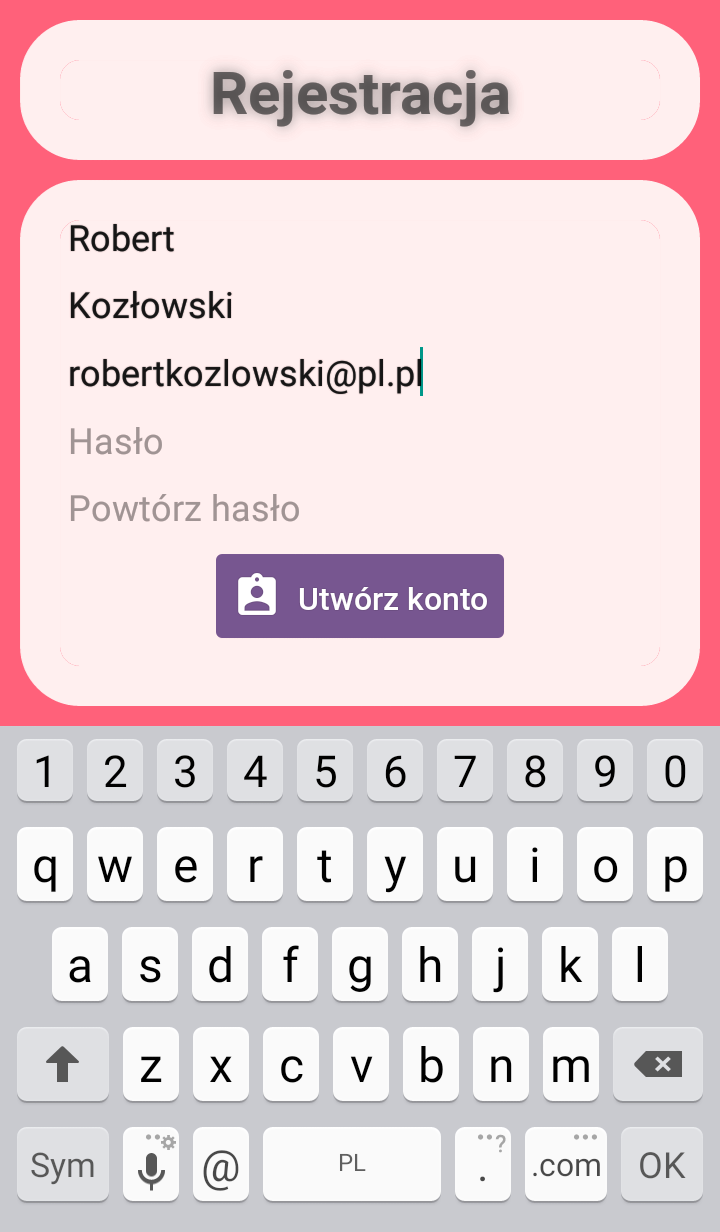
\includegraphics[width=\linewidth]{rejestracja2.png}
    \end{framed}
    \caption{Formularz rejestracyjny.}
  \end{subfigure}
  \begin{subfigure}[b]{0.4\linewidth}
    \begin{framed}
      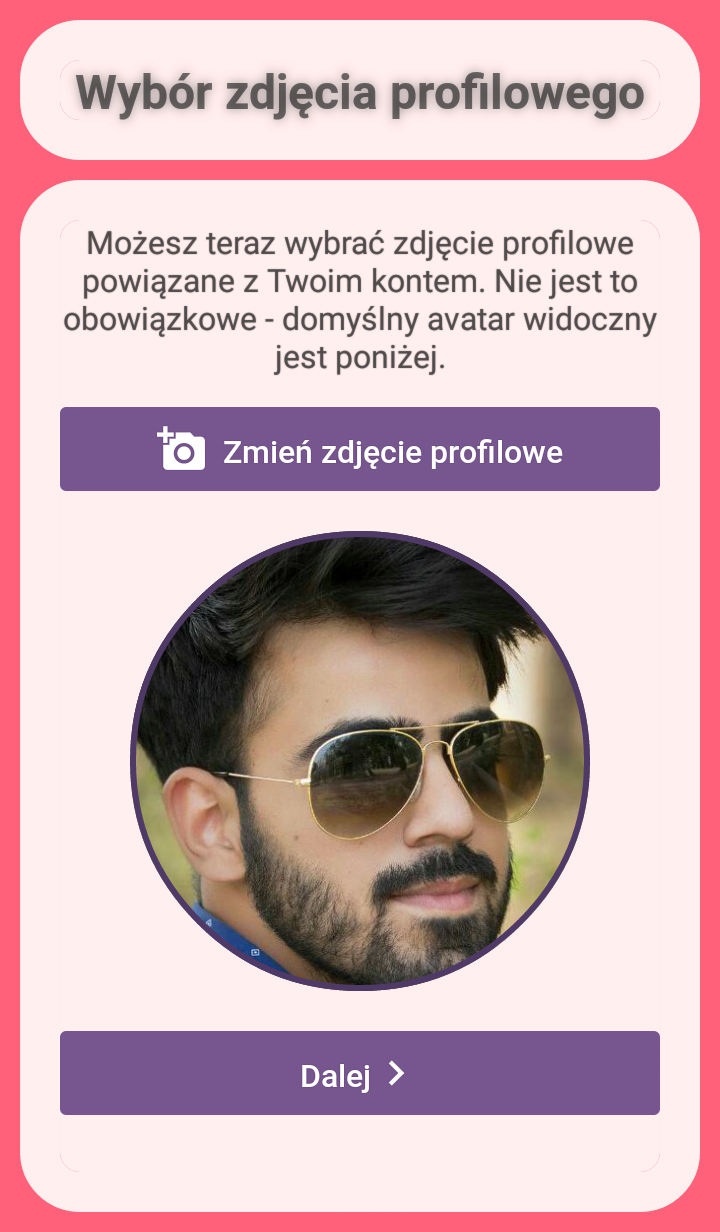
\includegraphics[width=\linewidth]{rejestracja3.png}
    \end{framed}
    \caption{Wybór zdjęcia profilowego.}
  \end{subfigure}
  \caption{Proces rejestracji nowego konta.}
  \label{fig:registration}
\end{figure}

\section{Dodawanie nowego ogłoszenia}
    \subsection{Krótki opis}
    Wprowadzenie przez użytkownika informacji potrzebnych do stworzenia nowego ogłoszenia oraz opublikowanie go na liście aktualnie dostępnych
    ogłoszeń.
    \subsection{Cele}
    Zapewnienie możliwości przeglądania nowo utworzonego ogłoszenia innym użytkownikom aplikacji.
    \subsection{Warunki wstępne}
    \begin{itemize}
        \item Aplikacja jest zainstalowana na urządzeniu użytkownika.
        \item Użytkownik posiada poprawnie założone konto.
        \item Użytkownik jest zalogowany w aplikacji.
        \item Użytkownik dysponuje stabilnym połączeniem internetowym.
    \end{itemize}
    \subsection{Czynności}
    \subsubsection{Czynności podstawowe}
    \begin{enumerate}
        \item Użytkownik naciska oznaczony przycisk, który rozwija szufladkowe menu.
        \item Użytkownik wskazuje w menu pozycję ``Dodaj nowe ogłoszenie''.
        \item Na ekranie pojawia się formularz dodawania ogłoszenia z podpisanymi polami.
        \item Użytkownik wprowadza (w dowolnej kolejności) wymagane informacje:
        \begin{itemize}
            \item Tytuł ogłoszenia, który będzie widoczny na liście ogłoszeń
            \item Właściwa treść ogłoszenia
            \item Sugerowana data przydatności do spożycia
            \begin{itemize}
                \item Użytkownik otwiera okienko kalendarza z graficznym rozkładem dni bieżącego miesiąca.
                \item W razie potrzeby użytkownik przechodzi za pomocą przycisków-strzałek do dalszych miesięcy.
                \item Użytkownik wskazuje konkretny dzień w kalendarzu.
            \end{itemize}
            \item Preferowany adres odbioru (z rozwijanej listy uprzednio zapisanych w aplikacji miejsc odbioru)
            \item Kategoria ogłoszenia (np.\ pieczywo, mięso, warzywa, dania pasteryzowane\ldots)
            \begin{itemize}
                \item Użytkownik rozwija listę dostępnych kategorii.
                \item Użytkownik wskazuje kategorię, która wydaje się najbardziej odpowiednia do zawartości ogłoszenia.
            \end{itemize}
            \item Hasztagi przypisane do ogłoszenia (np. \texttt{\#bezglutenu}, \texttt{\#mięsne}, \texttt{\#słodkie},\\ \texttt{\#wegetariańskie}\ldots)
            \begin{itemize}
                \item Użytkownik rozwija listę dostępnych hasztagów.
                \item Użytkownik wybiera (być może wiele) hasztagów pasujących do ogłoszenia.
                \item Dostępna jest także wyszukiwarka hasztagów.
            \end{itemize}
        \end{itemize}
        \item Użytkownik przesuwa widok ekranu na koniec formularza i naciska przycisk ``Dodaj ogłoszenie''.
        \item Aplikacja komunikuje się z serwerem, wysyłając prośbę o dodanie wprowadzonego ogłoszenia do bazy danych.
        \item Aplikacja otrzymuje odpowiedź od serwera --- ogłoszenie zostało dodane pomyślnie.
        \item Użytkownik dostaje informację zwrotną: aplikacja wyświetla na ekranie listę ogłoszeń użytkownika z nowo dodanym ogłoszeniem na szczycie listy.
    \end{enumerate}
    \subsubsection{Czynności alternatywne}
    Użytkownik może opcjonalnie dodać zdjęcia artykułu żywnościowego, opakowania, etykiet.
    \begin{enumerate}
        \item Użytkownik wskazuje przycisk ``Dodaj nowe zdjęcie''.
        \item Aplikacja wyświetla okienko z prośbą o wskazanie źródła zdjęcia, do wyboru: załączenie zdjęcia z pamięci urządzenia (galerii)
        lub utworzenie aparatem nowego zdjęcia.
        \begin{itemize}
            \item Jeżeli użytkownik wyrazi chęć dodania istniejącego zdjęcia, aplikacja uruchamia klasyczny interfejs przeglądania galerii
            systemu operacyjnego.
            \item Wybór opcji zrobienia nowego zdjęcia przekazuje sterowanie wbudowanej w system operacyjny aplikacji obsługującej aparat.
        \end{itemize}
        \item Jeżeli zdjęcie ma zbyt duży rozmiar, następuje jego kompresja (po stronie aplikacji).
        \item Na ekranie formularza pojawia się miniaturka dodanego zdjęcia.
    \end{enumerate}
    \subsubsection{Czynności niepoprawne}
    We wszystkich wymienionych poniżej przypadkach na ekranie wyświetla się okienko ze stosownym komunikatem. Użytkownik zostaje przekierowany z powrotem do ekranu edycji formularza, aby mógł wprowadzić zmiany.
    \begin{enumerate}
        \item Użytkownik nie wprowadził kompletu wymaganych informacji.
        \item Wartości niektórych pól formularza nie spełniają kryteriów akceptacji (np.\ zbyt mała liczba wskazanych hasztagów)
        \item Nastąpił błąd komunikacji z serwerem --- prośba o dodanie ogłoszenia nie została rozpatrzona.
        \item Serwer zasygnalizował błąd podczas operacji dodawania ogłoszenia do bazy danych.
    \end{enumerate}
    \subsection{Możliwe rozwinięcia}
    \subsubsection{Automatyczna klasyfikacja ogłoszeń}
    Wyświetlenie podpowiedzi co do wyboru odpowiedniej kategorii na podstawie analizy słownictwa użytego w treści ogłoszenia.

\newpage
\begin{figure}[H]
  \centering

  \begin{subfigure}[b]{0.4\linewidth}
    \begin{framed}
      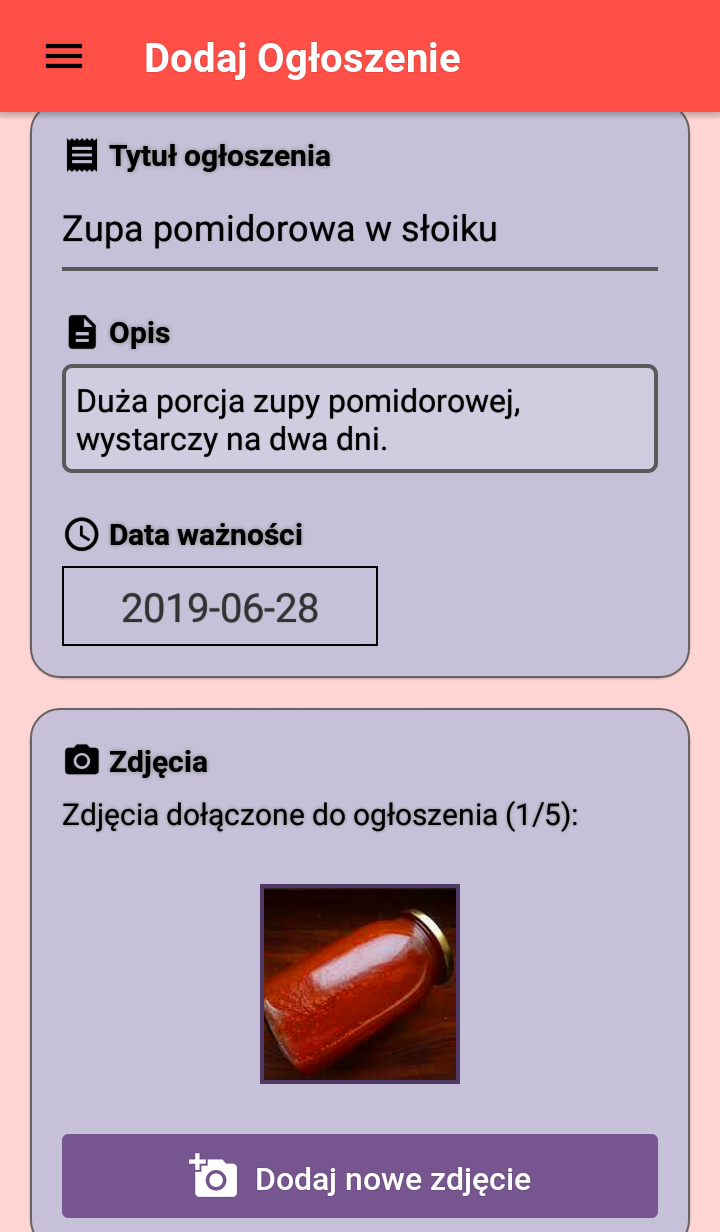
\includegraphics[width=\linewidth]{dodawanie1.png}
    \end{framed}
  \end{subfigure}
  \begin{subfigure}[b]{0.4\linewidth}
    \begin{framed}
      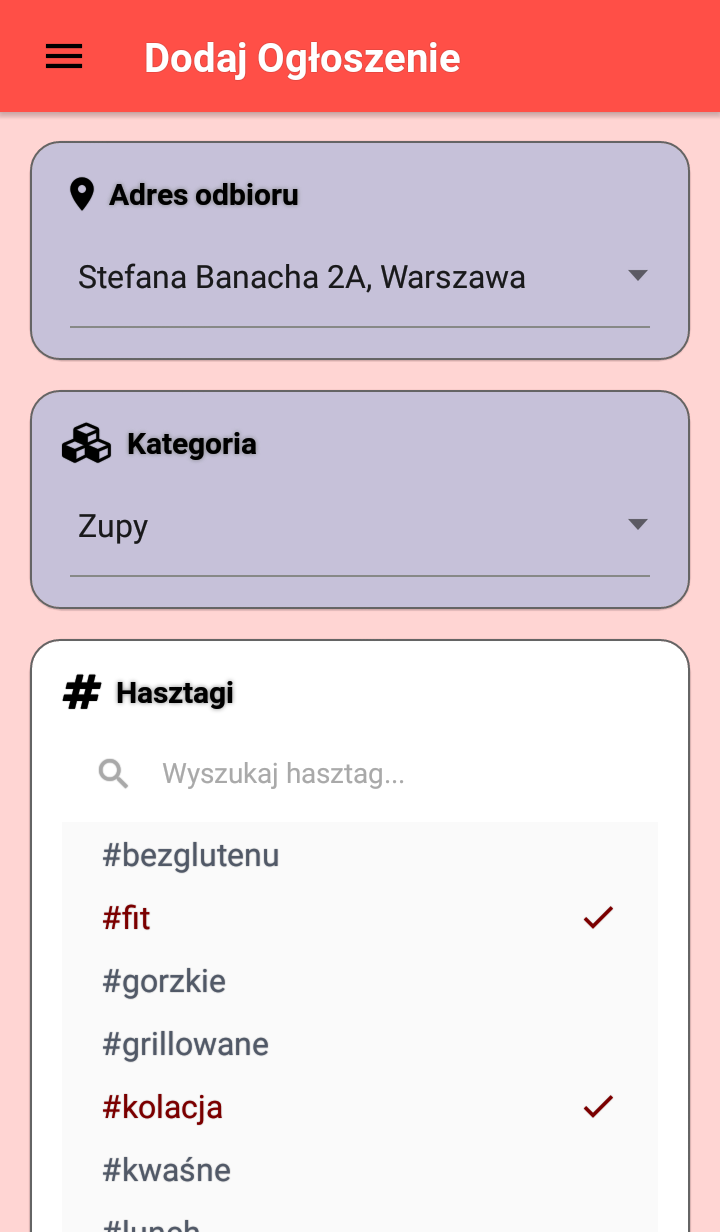
\includegraphics[width=\linewidth]{dodawanie2.png}
    \end{framed}
  \end{subfigure}
  \caption{Formularz dodawania nowego ogłoszenia.}
  \label{fig:addoffer}
\end{figure}

\section{Konwersacja (czat) z innym użytkownikiem}
    \subsection{Krótki opis}
    Wykorzystanie funkcji czatu do komunikacji z innym użytkownikiem aplikacji.
    \subsection{Cele}
    \begin{itemize}
        \item Możliwość zadawania wystawcy ogłoszenia dodatkowych pytań.
        \item Udostępnienie prywatnego kanału do ustalania szczegółów odbioru produktu.
        \item Zachęcenie użytkowników aplikacji do współtworzenia aktywnej społeczności.
    \end{itemize}
    \subsection{Warunki wstępne}
    \begin{itemize}
        \item Aplikacja jest zainstalowana na urządzeniu użytkownika.
        \item Użytkownik posiada poprawnie założone konto.
        \item Użytkownik jest zalogowany w aplikacji.
        \item Użytkownik dysponuje stabilnym połączeniem internetowym.
    \end{itemize}
    \subsection{Czynności}
    \subsubsection{Czynności podstawowe}
    \begin{enumerate}
        \item Użytkownik A otwiera ekran czatu z użytkownikiem B. Może to zrobić na kilka sposobów:
        \begin{itemize}
            \item Naciskając przycisk ``Otwórz czat z wystawiającym'' widocznego na ekranie ogłoszenia wystawionego przez B.
            \item Wybierając opcję ``Nowy czat'' w sekcji \textit{Czaty}.
            \item Wskazując awatar użytkownika B w sekcji \textit{Czaty} (jeżeli użytkownicy A oraz B rozmawiali ze sobą wcześniej).
        \end{itemize}
        \item W dolnej części ekranu pojawia się pole tekstowe do wpisania wiadomości oraz przycisk służący do jej wysłania. Jeżeli użytkownicy A i B rozmawiali ze sobą wcześniej, na ekranie będzie także widoczna przewijana lista poprzednich wiadomości, uporządkowana chronologicznie.
        \item Użytkownik A wpisuje treść wiadomości i wysyła ją.
        \item Nowa wiadomość zostaje dopisana do prowadzonej historii konwersacji.
        \item Użytkownik A oczekuje na odpowiedź użytkownika B:\@
        \begin{itemize}
            \item Jeżeli osoba B udzieli odpowiedzi od razu, jej treść pojawi się na ekranie użytkownika A w czasie rzeczywistym.
            \item W przypadku, gdy użytkownik A nie korzysta w danej chwili z aplikacji ``Podziel się'' w systemie Android, otrzyma powiadomienie (notyfikację) systemu operacyjnego o~nowej wiadomości od użytkownika B.
        \end{itemize}
    \end{enumerate}
    \subsubsection{Czynności niepoprawne}
    \begin{enumerate}
        \item Nastąpił błąd komunikacji z serwerem --- nie udało się wysłać wiadomości.
        \item Serwer zasygnalizował błąd podczas dopisywania wiadomości do historii konwersacji.
    \end{enumerate}
    \subsection{Możliwe rozwinięcia}
    \subsubsection{Przesyłanie obrazów}
    Umożliwienie przesyłania wiadomości w formie zdjęć. W tym celu użytkownik wysyłający wiadomość mógłby wybrać piktogram ``prześlij obraz''. Dalszy scenariusz byłby analogiczny do opisanego w \textit{Czynnościach alternatywnych} z punktu 3.2.4.

\newpage
\begin{figure}[H]
  \centering
  \begin{subfigure}[b]{0.4\linewidth}
    \begin{framed}
      
\includegraphics[width=\linewidth]{czat.png}
    \end{framed}
  \end{subfigure}
  \caption{Ekran czatu.}
  \label{fig:chat}
\end{figure}

\section{Ocena innego użytkownika}
    \subsection{Krótki opis}
    Wystawienie innemu użytkownikowi oceny w skali od 1 do 6 oraz możliwość napisania krótkiego komentarza dotyczącego współpracy z nim.
    \subsection{Cele}
    Informowanie innych użytkowników o jakości współpracy z daną osobą, w szczególności ostrzeganie innych przed nierzetelnymi użytkownikami.
    \subsection{Warunki wstępne}
    \begin{itemize}
        \item Aplikacja jest zainstalowana na urządzeniu użytkownika.
        \item Użytkownik posiada poprawnie założone konto.
        \item Użytkownik jest zalogowany w aplikacji.
        \item Użytkownik dysponuje stabilnym połączeniem internetowym.
    \end{itemize}
    \subsection{Czynności}
    \subsubsection{Czynności podstawowe}
    \begin{enumerate}
        \item Użytkownik A otwiera publiczny profil użytkownika B (zwykle poprzez naciśnięcie zdjęcia profilowego na ekranie ogłoszenia, które użytkownik B wystawił).
        \item Wyświetla się ekran z profilem użytkownika B, a na nim następujące elementy:
        \begin{itemize}
            \item Imię oraz nazwisko użytkownika.
            \item Zdjęcie profilowe.
            \item Licznik osób obserwujących.
            \item Przycisk ``Obserwuj'' / ``Przestań obserwować''.
            \item Zbiorcza ocena innych użytkowników w skali od 1 do 6.
            \item Sześciogwiazdkowa skala własnej oceny.
            \item Pole tekstowe przeznaczone na wpisanie komentarza.
            \item Przycisk ``Wyślij opinię’’.
            \item Lista opinii i komentarzy wystawionych przez społeczność użytkowników.
        \end{itemize}
        \item Użytkownik A ocenia użytkownika B w skali od 1 do 6.
        \item Użytkownik A wpisuje krótki komentarz odnośnie użytkownika B.
        \item Użytkownik A naciska przycisk ``Wyślij opinię’’.
    \end{enumerate}
    \subsubsection{Czynności alternatywne}
    Użytkownik A może co najwyżej raz ocenić użytkownika B. Jeśli miało już to miejsce, użytkownik A może edytować swoją ocenę na sześciostopniowej skali. Istnieje jednak możliwość wielokrotnego wystawiania komentarzy (np.\ dla każdego ogłoszenia B oddzielnie).
    \subsubsection{Czynności niepoprawne}
    \begin{enumerate}
        \item Nastąpił błąd komunikacji z serwerem --- prośba o dodanie / edycję opinii nie została rozpatrzona.
        \item Serwer zasygnalizował błąd podczas operacji dodawania / edycji opinii w bazie danych.
    \end{enumerate}
    \subsection{Możliwe rozwinięcia}
    Blokada możliwości oceny danego użytkownika do momentu, w którym odbierzemy od niego (lub on od nas) produkt z przynajmniej jednego ogłoszenia.

\newpage
\begin{figure}[H]
  \centering

  \begin{subfigure}[b]{0.4\linewidth}
    \begin{framed}
      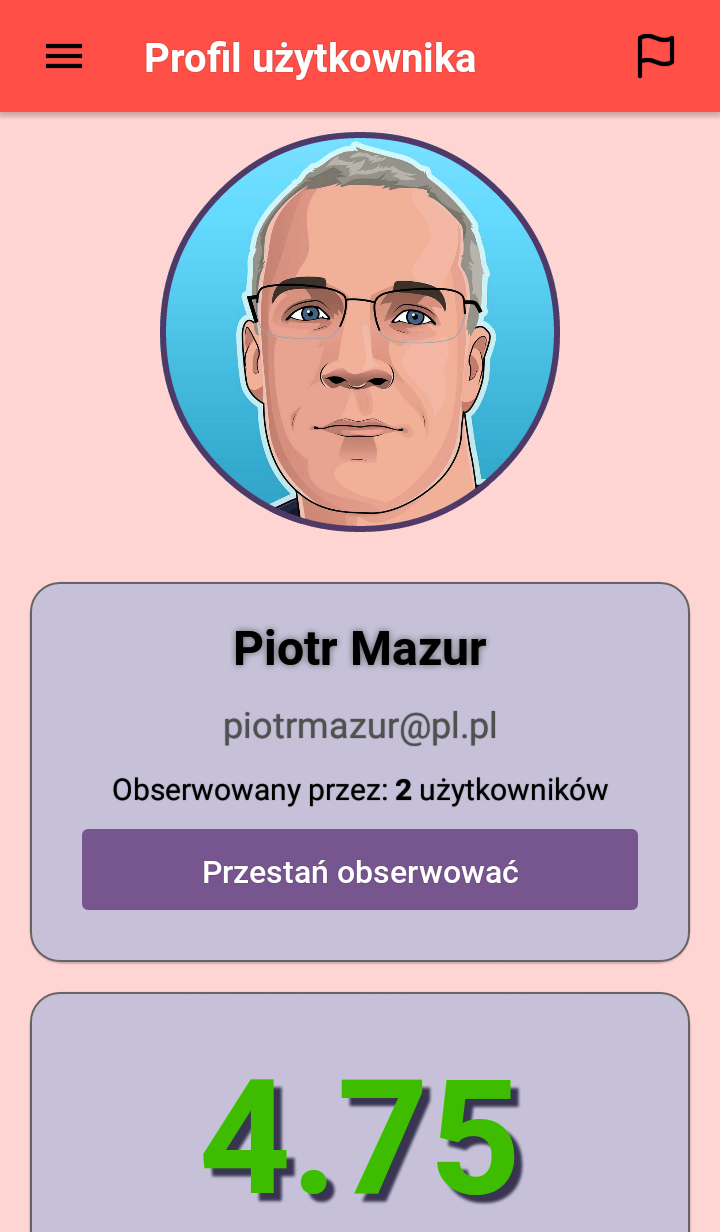
\includegraphics[width=\linewidth]{profil1.png}
    \end{framed}
  \end{subfigure}
  \begin{subfigure}[b]{0.4\linewidth}
    \begin{framed}
      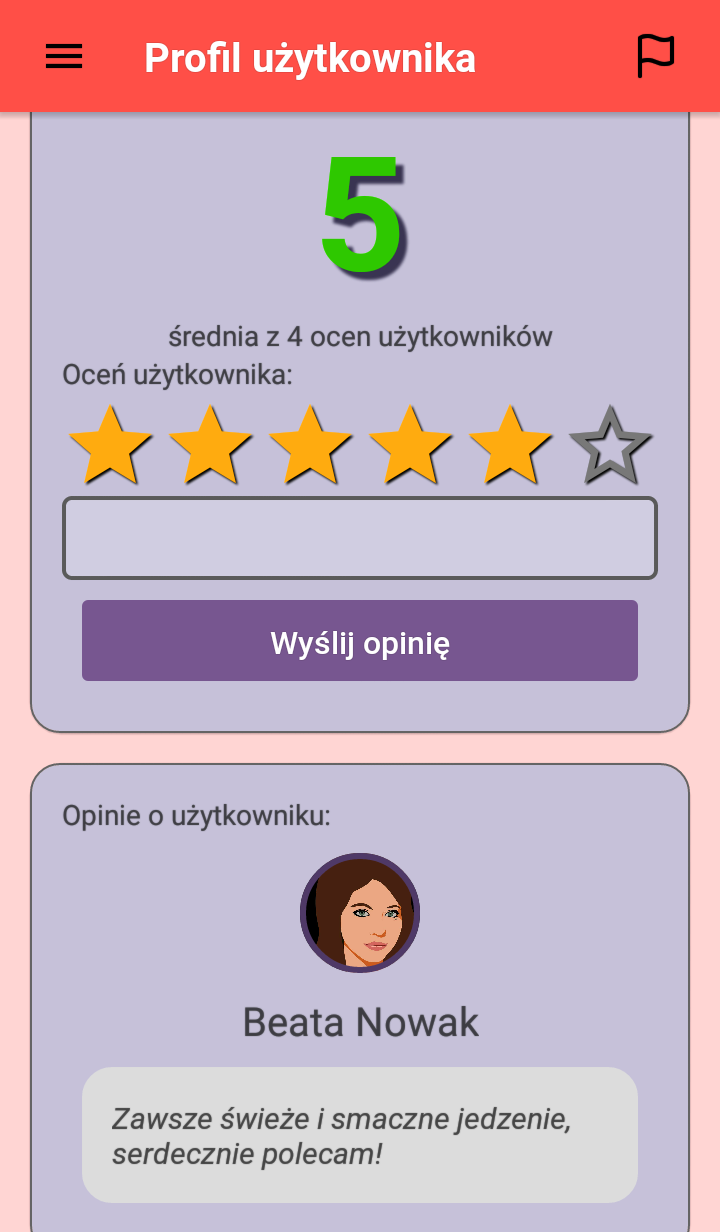
\includegraphics[width=\linewidth]{profil2.png}
    \end{framed}
  \end{subfigure}
  \caption{Profil użytkownika.}
  \label{fig:grading}
\end{figure}

\section{Odbiór produktów oferowanych na liście ogłoszeń}
    \subsection{Krótki opis}
    Umożliwienie użytkownikowi, który jest zainteresowany odbiorem przedmiotu z ogłoszenia (A) oraz użytkownikowi, który wystawił ogłoszenie (B) wspólnego ustalenia szczegółów odbioru.
    \subsection{Cele}
    \begin{itemize}
        \item Umożliwienie użytkownikom ustalenia szczegółów odbioru produktu (takich jak termin odbioru czy miejsce odbioru).
        \item Łatwiejsze zarządzanie statusem ogłoszeń.
    \end{itemize}
    \subsection{Warunki wstępne}
    \begin{itemize}
        \item Aplikacja jest zainstalowana na urządzeniach użytkowników A i B.
        \item Użytkownicy posiadają poprawnie założone konta.
        \item Użytkownicy są zalogowani w aplikacji.
        \item Użytkownik B dodał ogłoszenie.
        \item Użytkownicy dysponują stabilnym połączeniem internetowym.
    \end{itemize}
    \subsection{Czynności}
    \subsubsection{Czynności podstawowe}
    \paragraph{Użytkownik A}
    \begin{enumerate}
        \item Użytkownik otwiera listę dostępnych ogłoszeń i wskazuje jedno z nich.
        \item Na ekranie ze szczegółami ogłoszenia użytkownik naciska przycisk \textit{``Otwórz czat z wystawiającym''}.
        \item Użytkownikowi otwiera się ekran czatu z autorem ogłoszenia.
        \item Użytkownik wysyła wiadomość, w której wyraża chęć odbioru produktu z ogłoszenia.
        \item Jeżeli użytkownik otrzyma odpowiedź pozytywną, użytkownicy ustalają między sobą szczegóły odbioru.
    \end{enumerate}
    \paragraph{Użytkownik B}
    \begin{enumerate}
        \item Użytkownik otrzymuje nową wiadomość na czacie z chęcią odbioru oferowanego produktu.
        \item Użytkownik decyduje, czy chce oddać oferowany produkt użytkownikowi A\@:
        \begin{itemize}
            \item Jeżeli B nie chce oddać produktu użytkownikowi A, wysyła wiadomość odmowną i interakcja się kończy.
            \item Jeżeli B chce oddać produkt, wysyła wiadomość pozytywną, interakcja trwa dalej.
        \end{itemize}
        \item Użytkownicy ustalają między sobą szczegóły odbioru.
        \item Po oddaniu oferowanego produktu, użytkownik naciska przycisk \textit{``Oznacz jako odebrane''} na ekranie szczegółów swojego ogłoszenia, dzięki czemu produkt zniknie z listy dostępnych ogłoszeń. Podczas tej operacji użytkownik musi wskazać, dla kogo została dokonana rezerwacja.
    \end{enumerate}
    \subsubsection{Czynności alternatywne}
    Jeżeli użytkownik chciałby wycofać ogłoszenie z listy, może nacisnąć przycisk \textit{``Usuń ogłoszenie''}.
    \subsubsection{Czynności niepoprawne}
    \begin{enumerate}
        \item Czynności niepoprawne z podpunktu 3.3.4 dotyczące funkcjonalności czatu.
        \item Nastąpił błąd komunikacji z serwerem --- prośba o oznaczenie ogłoszenia jako oddane nie została rozpatrzona.
        \item Serwer zasygnalizował błąd podczas operacji związanej z oznaczeniem ogłoszenia jako oddane.
    \end{enumerate}

\newpage
\begin{figure}[H]
  \centering
  \begin{subfigure}[b]{0.4\linewidth}
    \begin{framed}
      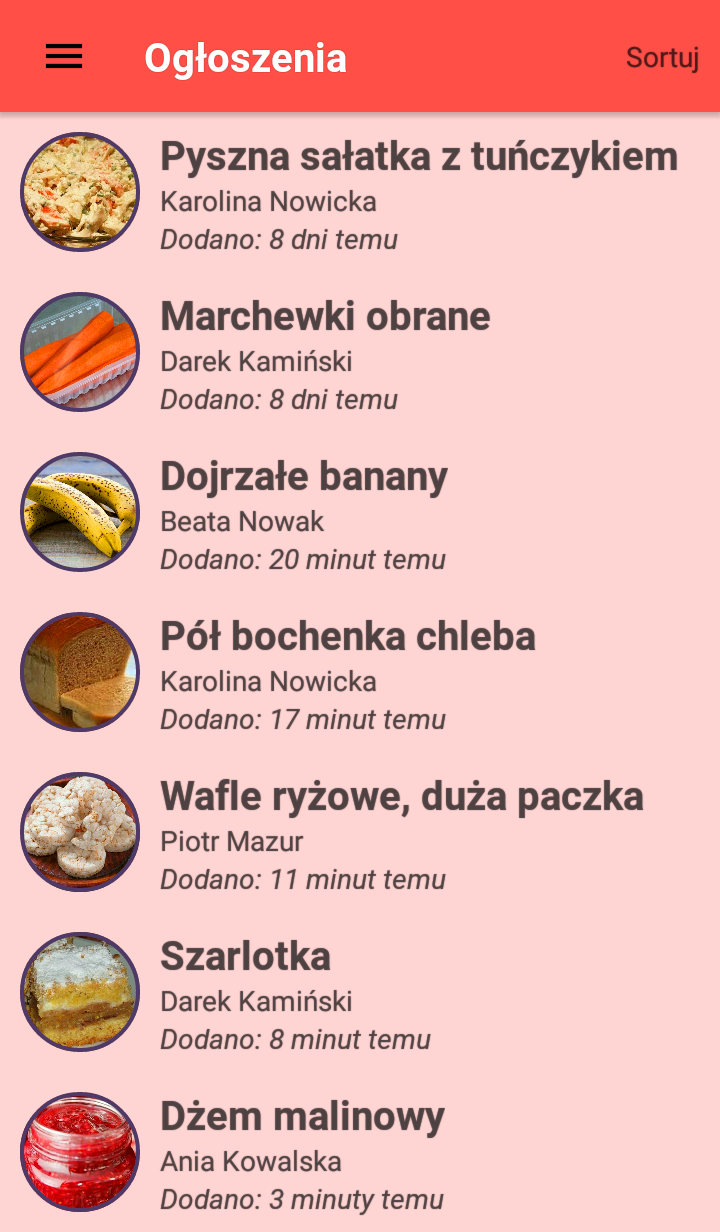
\includegraphics[width=\linewidth]{lista.png}
    \end{framed}
  \end{subfigure}
  \caption{Lista dostępnych ogłoszeń.}
  \begin{subfigure}[b]{0.4\linewidth}
    \begin{framed}
      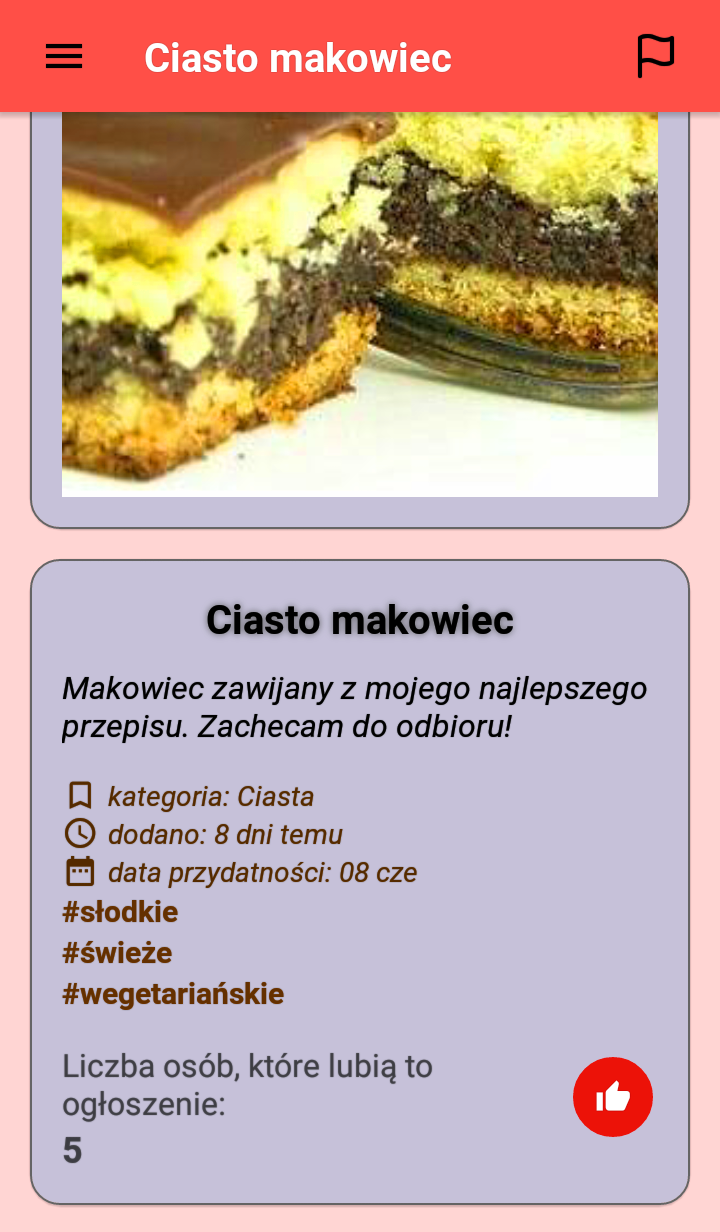
\includegraphics[width=\linewidth]{szczegoly1.png}
    \end{framed}
  \end{subfigure}
  \begin{subfigure}[b]{0.4\linewidth}
    \begin{framed}
      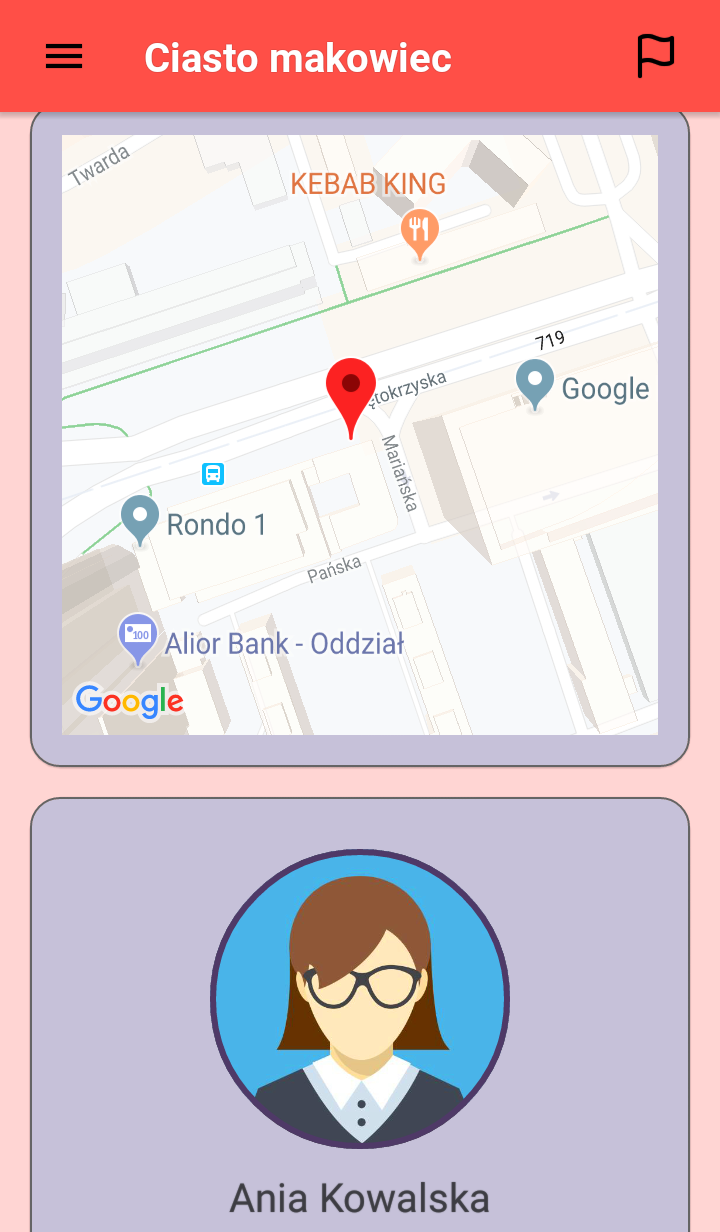
\includegraphics[width=\linewidth]{szczegoly2.png}
    \end{framed}
  \end{subfigure}
  \caption{Szczegóły ogłoszenia.}
  \label{fig:offerdetails}
\end{figure}

\chapter{Zarządzanie projektem}\label{r:zarzadzanieProjektem}
\section{Wykorzystane narzędzia}

W trakcie prac nad projektem głównym kanałem komunikacji był portal Slack. Wykorzystywany był zarówno do komunikacji między członkami zespołu, jak również między zespołem a zamawiającym. Dzięki niemu mogliśmy w łatwy sposób dzielić się plikami i dokumentami. Niezwykle pomocne okazała się również możliwość oznaczania postów z ważnymi informacjami, na przykład instrukcją dostępu do serwera.

Kod programu oraz tekst pracy licencjackiej przechowywane były w serwisie Github. Dzięki niemu mogliśmy również w prosty sposób spisywać listę zadań do zrobienia.

\section{Współpraca z zamawiającą}
Współpraca z zamawiającą była istotną częścią tego projektu. Pani Maria nie zna się na wytwarzaniu oprogramowania, nie wiedziała więc jakich informacji potrzebujemy. Aby się wzajemnie dobrze zrozumieć często komunikowaliśmy się, szczególnie na początku tworzenia aplikacji. Pani Maria na co dzień mieszka w Londynie, co utrudniło spotykanie się twarzą w twarz. Udało nam się tylko jedno takie spotkanie zorganizować (na początku współpracy), ale zaowocowało ono dość dokładnym spisem oczekiwanych funkcjonalności, dzięki któremu dalsza praca przebiegała bez większych wątpliwości. Przez cały czas regularnie kontaktowaliśmy się internetowo, w szczególności regularnie udostępnialiśmy zamawiającej aktualną wersję aplikacji aby upewnić się, że się dobrze rozumiemy. Dzięki temu ostatecznie udało nam się stworzyć aplikacje zgodną z oczekiwaniami zamawiającej.

\section{Organizacja pracy}

Nie korzystaliśmy w bezpośredni sposób z jednej ze znanych metodyk zarządzania projektami programistycznymi. Jednakże trzymaliśmy się kilku istotnych zasad. Przede wszystkim na bieżąco spisywaliśmy listę rzeczy do zrobienia. Staraliśmy się, żeby zadania były jak najmniejsze. Lista była aktualizowana co tydzień na zajęciach z przedmiotu zespołowy projekt programistyczny. Każdy z nas decydował jakie zadanie w danej chwili chce wykonać. Wspólnie zaprojektowaliśmy architekturę aplikacji oraz podejmowaliśmy najważniejsze decyzję dotyczące projektu. Na każdych zajęciach staraliśmy się na bieżąco omawiać problemy jakie w danej chwili napotykaliśmy.

Co ważne, nie dzieliliśmy zadań na te z części mobilnej i serwerowej. Pojedyncze zadanie dotyczyło najczęściej zaimplementowanie jakiejś funkcjonalności, na przykład dodawania zdjęć do ogłoszenia. Osoba odpowiedzialna za zadanie implementowała zarówno część dotyczącą aplikacji mobilnej jak i serwerowej. W ten sposób mogliśmy znacznie zrównoleglić prace nad projektem. Jedna osoba nie musiała czekać aż ktoś inny zrealizuje niezbędną pracę po stronie serwera. Ponad to uniknęliśmy w ten sposób nieporozumień związanych z działaniem nowo napisanego kodu. Co więcej każdy z nas, w równym stopniu, nauczył się zarówno tworzenia aplikacji mobilnej we frameworku ReactNative oraz realizacji części serwerowej we frameworku Django.

\section{Podział obowiązków}

\subsection{Kamil Ćwinatal}
\begin{itemize}
\setlength\itemsep{-0.2em}
    \item Widok listy ogłoszeń,
    \item Zdjęcia profilowe użytkowników,
    \item Zdjęcia ogłoszeń,
    \item Kategorie i hasztagi w ogłoszeniach,
    \item Dopracowanie ogólnego wyglądu aplikacji,
\end{itemize}{}

\subsection{Szymon Gajda}
\begin{itemize}
\setlength\itemsep{-0.2em}
    \item Dodawanie ogłoszeń,
    \item Dodanie lokalizacji do ogłoszeń,
    \item Wyświetlanie mapy w ogłoszeniach,
    \item Filtrowanie i sortowanie ogłoszeń po odległości między użytkownikiem a ogłoszeniem,
    \item Logowanie z Facebookiem,
    \item Zgłaszanie nieodpowiednich ogłoszeń,
\end{itemize}{}

\subsection{Paweł Giżka}
\begin{itemize}
\setlength\itemsep{-0.2em}
    \item Logowanie i rejestracja,
    \item Czat między użytkownikami,
    \item Powiadomienia,
    \item Sortowanie ogłoszeń,
    \item Możliwość obserwacji wybranych użytkowników,
    \item Konfiguracja serwera aplikacji,
\end{itemize}{}

\subsection{Tomasz Kanas}
\begin{itemize}
\setlength\itemsep{-0.2em}
    \item Widok szczegółów ogłoszenia,
    \item Widok własnych ogłoszeń,
    \item Widok profilu innych użytkowników,
    \item Ocenianie użytkowników,
    \item Widok i możliwość edycji własnego profilu,
\end{itemize}{}

\chapter{Zawartość płytki}\label{r:build}
\begin{tabbing}
      \hspace{20em} \=   \hspace{10em} \\
    /PodzielSieBackend/ \> Kod źródłowy części serwerowej. \\
    /PodzielSieBackend/README.md \> Instrukcja uruchamiania części serwerowej. \\
    /PodzielSieMobile/ \> Kod źródłowy części mobilnej. \\
    /PodzielSieModile/README.md \> Instrukcja uruchamiania części mobilnej. \\
    /PracaLicencjacka.pdf \> Praca licencjacka. \\
    /Precentacja.pdf \> Końcowa prezentacja projektu. \\
\end{tabbing}

\chapter{Podsumowanie}\label{r:pods}
W trakcie ostatnich siedmiu miesięcy powstała w pełni funkcjonalna aplikacja mobilna, która w istotny sposób może przyczynić się do zmniejszenia ilości marnowanej żywności. Udało nam się zrealizować zdecydowaną większość wymagań zamawiającej, w szczególności wszystkie niezbędne funkcjonalności zostały zaimplementowane.

W trakcie prac nad projektem nauczyliśmy się wielu zagadnień związanych z inżynierią oprogramowania, tworzeniem aplikacji mobilnych z wykorzystaniem ReactNative, implementacji części serwerowej we frameworku Django, integracji ze zewnętrznymi usługami czy administrowania serwerem aplikacyjnym. Było to dla nas również okazja do rozwinięciu tak zwanych umiejętności miękkich takich jak chociażby pracę w zespole czy kontakt z zamawiającym.

W chwili obecnej czekamy na informacje od zamawiającej dotyczące wdrożenia aplikacji do użytku. Niezależnie od tego czy aplikacja zostanie wdrożona, jesteśmy z niej bardzo zadowoleni. Realizacja tego projektu dała nam wiele satysfakcji.


\begin{thebibliography}{99}
\addcontentsline{toc}{chapter}{Bibliografia}

\bibitem[FAO]{fao} raport Organizacji Narodów Zjednoczonych do spraw Wyżywienia i Rolnictwa\\\textit{``Global food losses and food waste''}, \href{http://www.fao.org/3/mb060e/mb060e.pdf}{\texttt{fao.org/3/mb060e/mb060e.pdf}}

\bibitem[Eurostat]{eurostat} raport techniczny Komisji Europejskiej z 2010 roku\\\textit{``Preparatory Study on Food Waste Across EU 27''},\\\href{http://ec.europa.eu/environment/eussd/pdf/bio\_foodwaste\_report.pdf}{\texttt{ec.europa.eu/environment/eussd/pdf/bio\_foodwaste\_report.pdf}}

\bibitem[Kantar Millward Brown]{millward-brown}raport Federacji Polskich Banków Żywności \textit{``Nie marnuję jedzenia 2018''} z wynikami badań zrealizowanych przez Kantar Millward Brown,\\\href{http://bzsos.pl/2018/raportu-nie-marnuj-jedzenia-2018}{\texttt{bzsos.pl/2018/raportu-nie-marnuj-jedzenia-2018}}

\bibitem[Polityka]{polityka}opracowanie \textit{``Zgubione kalorie. Jak skutecznie walczyć z marnotrawieniem żywności''} dla magazynu Polityka Insight,\\\href{http://politykainsight.pl/gospodarka/ryzykaitrendy/\_resource/multimedium/20145149}{\texttt{politykainsight.pl/gospodarka/ryzykaitrendy/\_resource/multimedium/20145149}}

\bibitem[podzielmysie.pl]{podzielmysie} oficjalna strona akcji społecznej \textit{``Podziel się Posiłkiem z Bezdomnymi''}, \href{http://www.podzielmysie.pl}{\texttt{podzielmysie.pl}}

\bibitem[reducefoodwaste.eu]{rfw} oficjalna strona internetowa projektu Reduce Food Waste,\\
    \href{http://www.reducefoodwaste.eu}{\texttt{reducefoodwaste.eu}}

\bibitem[Olioex.com]{olio} Statystyki dotyczące wykorzystania żywności na świecie z oficjalnej strony aplikacji  \textit{Olio}, \href{https://olioex.com}{\texttt{olioex.com}}

\bibitem[toogoodtogo.com]{tgtg} Oficjalna strona aplikacji \textit{Too Good To Go}, \href{https://toogoodtogo.com}{\texttt{toogoodtogo.com}}.

\bibitem[ec.europa.eu]{ec} Działania KE ws.\ marnowania żywności\\ \href{https://ec.europa.eu/food/safety/food_waste_en}{\texttt{https://ec.europa.eu/food/safety/food\_waste\_en}}

\bibitem[IDC]{popluarnoscAndroid} Popularność systemu Android w Polsce\\
\href{https://www.telepolis.pl/wiadomosci/prawo-finanse-statystyki/w-2017-roku-w-polsce-sprzedano-8-8-mln-smartfonow}{https://www.telepolis.pl/wiadomosci/prawo-finanse-statystyki/w-2017-roku-w-polsce-sprzedano-8-8-mln-smartfonow}

\bibitem[ReactNative]{reactnative} \href{https://facebook.github.io/react-native/}{\texttt{facebook.github.io/react-native}}

\bibitem[GoogleMaps]{googlemaps} \href{https://developers.google.com/maps/documentation/}{\texttt{developers.google.com/maps/documentation}}

\bibitem[Firebase]{firebase} \href{https://firebase.google.com/docs/cloud-messaging/}{\texttt{firebase.google.com/docs/cloud-messaging}}

\bibitem[Notifications]{nots} \href{https://developer.apple.com/notifications/}{\texttt{developer.apple.com/notifications}}

\bibitem[AWS]{amazonaws} \href{https://aws.amazon.com/}{\texttt{aws.amazon.com}}

\bibitem[Django]{django} \href{https://www.djangoproject.com/}{\texttt{djangoproject.com}}

\bibitem[Gunicorn]{gunicorn} \href{https://gunicorn.org/}{\texttt{gunicorn.org}}

\bibitem[NginX]{nginx} \href{https://www.nginx.com/}{\texttt{nginx.com}}

\bibitem[PostgreSQL]{postgresql} \href{https://www.postgresql.org/}{\texttt{postgresql.org}}


\bibitem[Framework]{framework} \href{https://pl.wikipedia.org/wiki/Framework}{\texttt{https://pl.wikipedia.org/wiki/Framework}}

\end{thebibliography}

\end{document}


%%% Local Variables:
%%% mode: latex
%%% TeX-master: t
%%% coding: latin-2
%%% End:

